%\section{Competition Results and Analysis}
%\label{sec:results}





\section{Experimental Setup} 
\label{sec:exp-set}
The solvers were run on the StarExec platform~\cite{starexec} with a dedicated cluster of 12 nodes, where each node
consisted of two 4-core 2.4GHz Intel processors with 256GB RAM and a 1TB hard drive. The memory
usage limit of each solver run was set to 128GB. The wallclock time limit was set to 3600 seconds (thus,
a solver that used all cores could consume at most 14400 seconds cpu time).
The solutions that the solvers produce are being checked for both syntactic and semantic correctness.
That is, a first post-processor checks that the produced expression adheres to the grammar specified in
the given benchmark, and if this check passes, a second post-processor checks that the solution adheres
to semantic constraints given in the benchmark (by invoking an SMT solver).




\section{Results Overview}
\label{sec:comp-results}
The combined results for all tracks are given in Figure~\ref{fig:combinedresults}. The figure shows the sum of benchmarks solved by the solvers for each track. We can observe that the $\eusolvernew$ solved the highest number of benchmarks in the combined tracks, and   the \euphony\ solver and the $\cvcnew$ solver  solved almost as many.


\begin{figure}
	\centering
	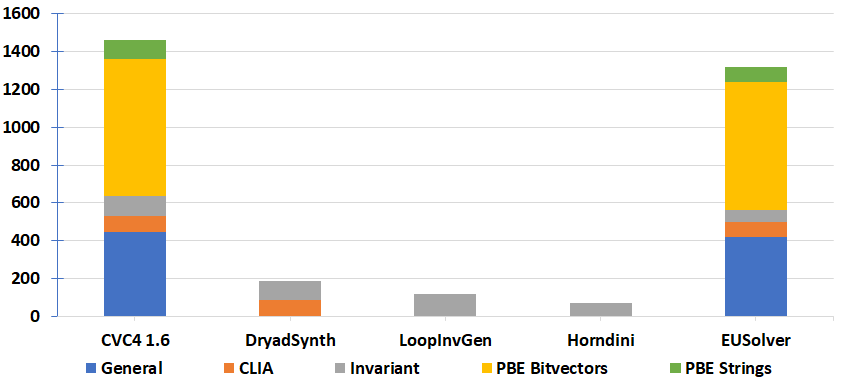
\includegraphics[scale=0.5]{Figures/TotalSolved.pdf}
	\caption{The overall combined results for each solver on benchmarks from all five tracks.}
	\label{fig:combinedresults}
\end{figure}



The primary criterion for winning a track was the number of benchmarks solved, but we also analyzed the time to solve and the the size of the generated expressions. Both where classified using a pseudo-logarithmic scale as follows.
For time to solve the scale is [0,1), [1,3), [3,10), [10,30),[30, 100), [100,300), [300, 1000), [1000,3600), $>$3600. That is the first ``bucket'' refers to termination in less than one second, the second to termination in one to three second and so on. We say that a solver solved a certain benchmark \emph{among the fastest} if the time it took to solve that benchmark was on the same bucket as that of the solver who solved that benchmark the fastest. 
For the expression sizes the pseudo-logarithmic scale we use is [1,10), [10,30), [30,100), [100,300), [300,1000), $>$1000 where expression size is the number of nodes in the SyGuS parse-tree.
In some tracks there was a tie or almost a tie in terms of the number of solved benchmarks, but the differences in the time to solve where significant.
We also report on the number of benchmarks \emph{solved uniquely} by a solver (meaning the number of benchmark that solver was the single solver that managed to solve them).



Figure~\ref{fig:resultsPerTrack} shows the percentage of benchmarks solved by each of the solvers in each of the tracks (in the upper part) and the number of benchmarks solved among the fastest by each of the solvers in each of the tracks (in the lower part) and the number of benchmarks solved among the fastest. 

\begin{figure}
	\begin{center}
		\begin{minipage}{1\textwidth}
			\centering
			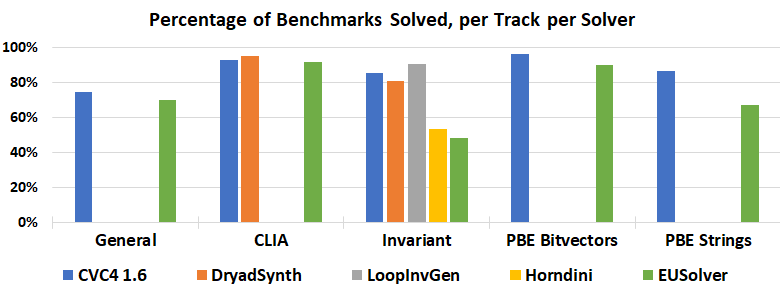
\includegraphics[scale=0.9,width=1\textwidth]{Figures/Solved.png}
		\end{minipage}
		\\
		\vspace{2mm}
		\begin{minipage}{1\textwidth}
			\centering
			\includegraphics[scale=0.9,width=1\textwidth]{Figures/Won.png}
		\end{minipage}
	\end{center}
	\caption{Percentage of benchmarks solved by the different solvers across all tracks, and the percentage of benchmarks a solver solved among the fastest for that benchmarks (according to the logarithmic scale)}\label{fig:resultsPerTrack}	
\end{figure}


\paragraph{General Track}
In the general track the \eusolvernew\ solved more benchmarks than all others (407), the \cvcnew\ came second, solving 378 benchmarks, and \euphony\ came third, solving 362 benchmarks. The same order appears in the number of benchmarks solved among the fastest: \eusolvernew\ with 276, \cvcnew\ with 236, and \euphony\ with 135. In terms of benchmarks solved uniquely by a solver, we have that \eusolvernew\ solved 34 uniquely, \cvcnew\ solved 9 uniquely, and \euphony\ solved 2 uniquely. 



\begin{table}[t]
	\begin{center}
		\scalebox{0.9}{
		\begin{tabular}{lr||rrrrrrrrrrrr|r}
			 &	& \rot{Compiler Optimizations and Bit Vectors}	& \rot{Let and Motion Planning} &	\rot{Invariant Generation with Bounded Ints} &	\rot{Invariant Generation with Unbounded Ints} &	\rot{Multiple Functions}	& \rot{Arrays} &	\rot{Hackers Delight} &	\rot{Integers} &	\rot{Program Repair} &	\rot{ICFP} &	\rot{Cryptographic Circuits} &	\rot{Instruction Selection} & {Total}\\\hline \hline
\multicolumn{2}{l||}{Number of benchmarks}  & 32 & 30 & 28 & 28 & 32 & 31 & 44 & 34 & 18 & 50 & 214 & 28 & 569 \\ \hline			 
\multirow{3}{*}{Solved} & \eusolvernew\ &	16	& 10	& 24	&24 &	18	& 31	& 35 &	33 &	14 &	50& 	152& 	0 & 407 \\
& \cvcnew\ &	15	& 15	& 24	& 24	& 12	& 31 &	44& 	34&	14&	48&	117&	0 & 378 \\
& \euphony\	& 19	&10 &	24 &	24 &	18	& 31	& 44	& 33	& 14	& 50	& 95 &	0 & 362 \\ \hline
\multirow{3}{*}{Fastest} & \eusolvernew\ &	7	&2 	& 12	& 14	& 6	& 5	& 20	& 14 &	13 &	40	& 143 &	0 & 276\\
 & \cvcnew &	11 &	15 &	18	& 19	& 9	& 31 &	44	& 33	& 7& 	19	& 30	& 0 & 236 \\
& \euphony	& 16 &	2	& 8	& 13 &	13 &	4	& 27 &	14 &	9	& 29	& 0& 	0 & 135 \\ \hline
\multirow{3}{*}{Uniquely} & \eusolvernew\ &	0	& 0& 	0	& 0& 	0	& 0& 	0	& 0 &	0	& 0	& 34 &	0 & 34 \\
& \cvcnew &	1	& 5&	0&	0&	1&	0	&0&	1&	1&	0	&0&	0 & 9\\
& \euphony	& 2	& 0	& 0& 	0	& 0& 	0	& 0& 	0	& 0& 	0 &	0	& 0 & 2\\ \hline			
		\end{tabular}}
	\end{center}
	\caption{Solvers performance across all categories of the general track}
	\label{tbl:general-categories}
\end{table}

We partition the benchmarks of the general track according to categories where different categories consists of related benchmarks. The results per category are given in the Table~\ref{tbl:general-categories}. We can see that \eusolvernew\ preformed better than others in the categories of program repair, icfp and cryptographic circuits. The \cvcnew\ solver preformed better than others in the categories of let and motion planning, invariant generation with bounded and unbounded integers, arrays, integers and hacker's delight. The \euphony\ solver preformed better than others in the categories of  multiple functions, compiler optimizations and bitvectors. We can also observe that none of the solvers could solve any of the instruction selection benchmarks. 




\begin{figure}
	\begin{center}
		\begin{minipage}{1\textwidth}
			\centering
			\includegraphics[scale=0.9,width=1\textwidth]{Figures/GeneralSolved.png}
		\end{minipage}
		\\
		\vspace{2mm}
		\begin{minipage}{1\textwidth}
			\centering
			\includegraphics[scale=0.9,width=1\textwidth]{Figures/GeneralWon.png}
		\end{minipage}
	\end{center}
	\caption{Percentage of benchmarks solved by the different solvers across all categories of the general track, and the percentage of benchmarks a solver solved among the fastest for that benchmark (according to the logarithmic scale).  }	
\end{figure}	


\paragraph{Conditional Linear Arithmetic Track}
In the CLIA track the \cvcnew\ solved all 73 benchmarks, \euphony\ and \eusolvernew\ solved 71 benchmarks, and \dryd\ solved 32 benchmarks. The \cvcnew\ solver solved 72 benchmarks among the fastest, followed by \eusolvernew\ which solved 29 among the fastest, \euphony\ which solved 11 among the fastetst, and \dryd\ which solved 3 among the fastest. None of the benchmarks where solved uniquely.

\paragraph{Invariant Generation Track}
In the invariant generation  track, both the \lig\ solver and the \cvcnew\ solver solved 65 out of 74 benchmarks, the \dryd\ solver solved 64 benchmarks, the Euphony solver solved 48 benchmarks and EUSolver solved 40 benchmarks. In terms of the time to solve the differences where more significant. The \lig\ solver solved 54 benchmarks among the fastest, followed by \cvcnew\ which solved 38 among the fastest, and \dryd\
which solved 36 among the fastest. There was one benchmark that only one solver solved, this is the \texttt{hola07.sl} benchmark, and the solver is \lig. 


\paragraph{Programming By Example BV Track}
In the PBE track using BV theory, the \ethree\ solver solved all 750 benchmarks, \euphony\ solved 747 benchmarks, \eusolvernew\ solved 242, benchmarks, and \cvcnew\ solved 687 benchmarks. The \ethree\ solver solved 692 among the fastest, \eusolvernew\ solved 211 among the fastest, \cvcnew\ solved 169 among the fastest, and \euphony\ solved 117 among the fastest. Three benchmarks where solved uniquely by \ethree, these are: \texttt{13_1000.sl}, \texttt{40_1000.sl} and \texttt{89_1000.sl}.

\paragraph{Programming By Example Strings Track}
In the PBE track using SLIA theory, the \cvcnew\ solved 89 out of 108 benchmarks, \euphony\ solved 78, and \eusolvernew\ solved 69. The \euphony\ solver solved 66 benchmarks among the fastest, \cvcnew\ solved 49 among the fastest and \eusolvernew\ solved 23 among the fastest. Nine benchmarks where solved by only one solver, which is \cvcnew.



\section{Detailed Results}
\label{sec:benchs-pres}
In the following section we show the results of the competition from the benchmark's perspective. 
For a given benchmark we would like to know: how many solvers solved it, what is the min and max time to solve,  what are the min and max size of the expressions produced, which solver solved the benchmark the fastest, and which solver produced the smallest expression.



We represents the results per benchmark in groups organized per tracks and categories. For instance, Fig.~\ref{fig:prog-rep-icfp} at the top presents details of the program repair benchmarks. The black bars show the range of the time to solve among the different solvers in pseudo logarithmic scale (as indicated on the upper part of the y-axis). Inspect for instance benchmark \texttt{t\_2.sl}. The black bar indicates that the fastest solver to solve it used less than 1 second, and the slowest used between 100 to 300 seconds. 
The black number above the black bar indicates the exact number of seconds (floor-rounded to the nearest second) it took the slowest solver to solve a benchmark (and $\infty$ if at least one solver exceeded the time bound). Thus, we can see that the slowest solver to solve \texttt{t\_2.sl} took 141 seconds to solve it. The white number at the lower part of the bar indicates the time of the fastest solver to solve that benchmark. Thus, we can see that the fastest solver to solve \texttt{t\_2.sl} required less than 1 second to do so. The colored squares/rectangles next to the lower part of the black bar, indicate which solvers were the fastest to solve that benchmark (according to the solvers' legend at the top). Here, \emph{fastest} means in the same logarithmic scale as the absolute fastest solver. For instance, we can see that \euphony\ and \eusolvernew\ were the fastest to solve \texttt{t\_2.sl}, solving it in less than a second
and that among the 2 solvers that solved \texttt{t\_3.sl} only \eusolvernew\ solved it in less than 1 seconds. 

Similarly, the gray bars indicate the range of expression sizes in pseudo logarithmic scales (as indicated on the lower part of the y-axis), where the size of an expression is determined by the number of nodes in its parse tree.
The black number at the bottom of the gray bar indicates the exact size expression of the largest solution (or $\infty$ if it exceeded 1000), and the white number at the top of the gray bar indicates the exact size expression of the smallest solution (when the smallest and largest size of expressions are in the same logarithmic bucket (as is the case in \texttt{t\_2.sl}), we provide only the largest expression size, thus there is no white number on the gray bar). The colored squares/rectangles next to the upper part of the gray bar indicates which solvers (according to the legend) produced the smallest expression (where \emph{smallest} means in the same logarithmic scale as the absolute smallest expression). For instance, for \texttt{t\_20.sl} the smallest expression produced had size 3, and 2 solvers out of the 3 who solved it managed to produce an expression of size less than 10.  

Finally, at the top of the figure above each benchmark there is a number indicating the number of solvers that solved that benchmark. For instance, one solver solved \texttt{t\_14.sl}, two solvers solved \texttt{t\_12.sl}, three solvers solved \texttt{t\_2.sl}, and no solver solved \texttt{t\_6.sl}. Note that the reason \texttt{t\_6.sl} has 2 as the upper time bound, is that that is the time to terminate rather than the time to solve. Thus, all solvers aborted within less than 2 seconds, but either they did not produce a result, or they produced an incorrect result. When no solver produced a correct result, there are no colored squares/rectangles next to the lower parts of the bars, as is the case for \texttt{t\_6.sl}.


\begin{figure*}
\noindent\makebox[\textwidth]{
	\scalebox{0.6}{
		\begin{tabular}{c}
			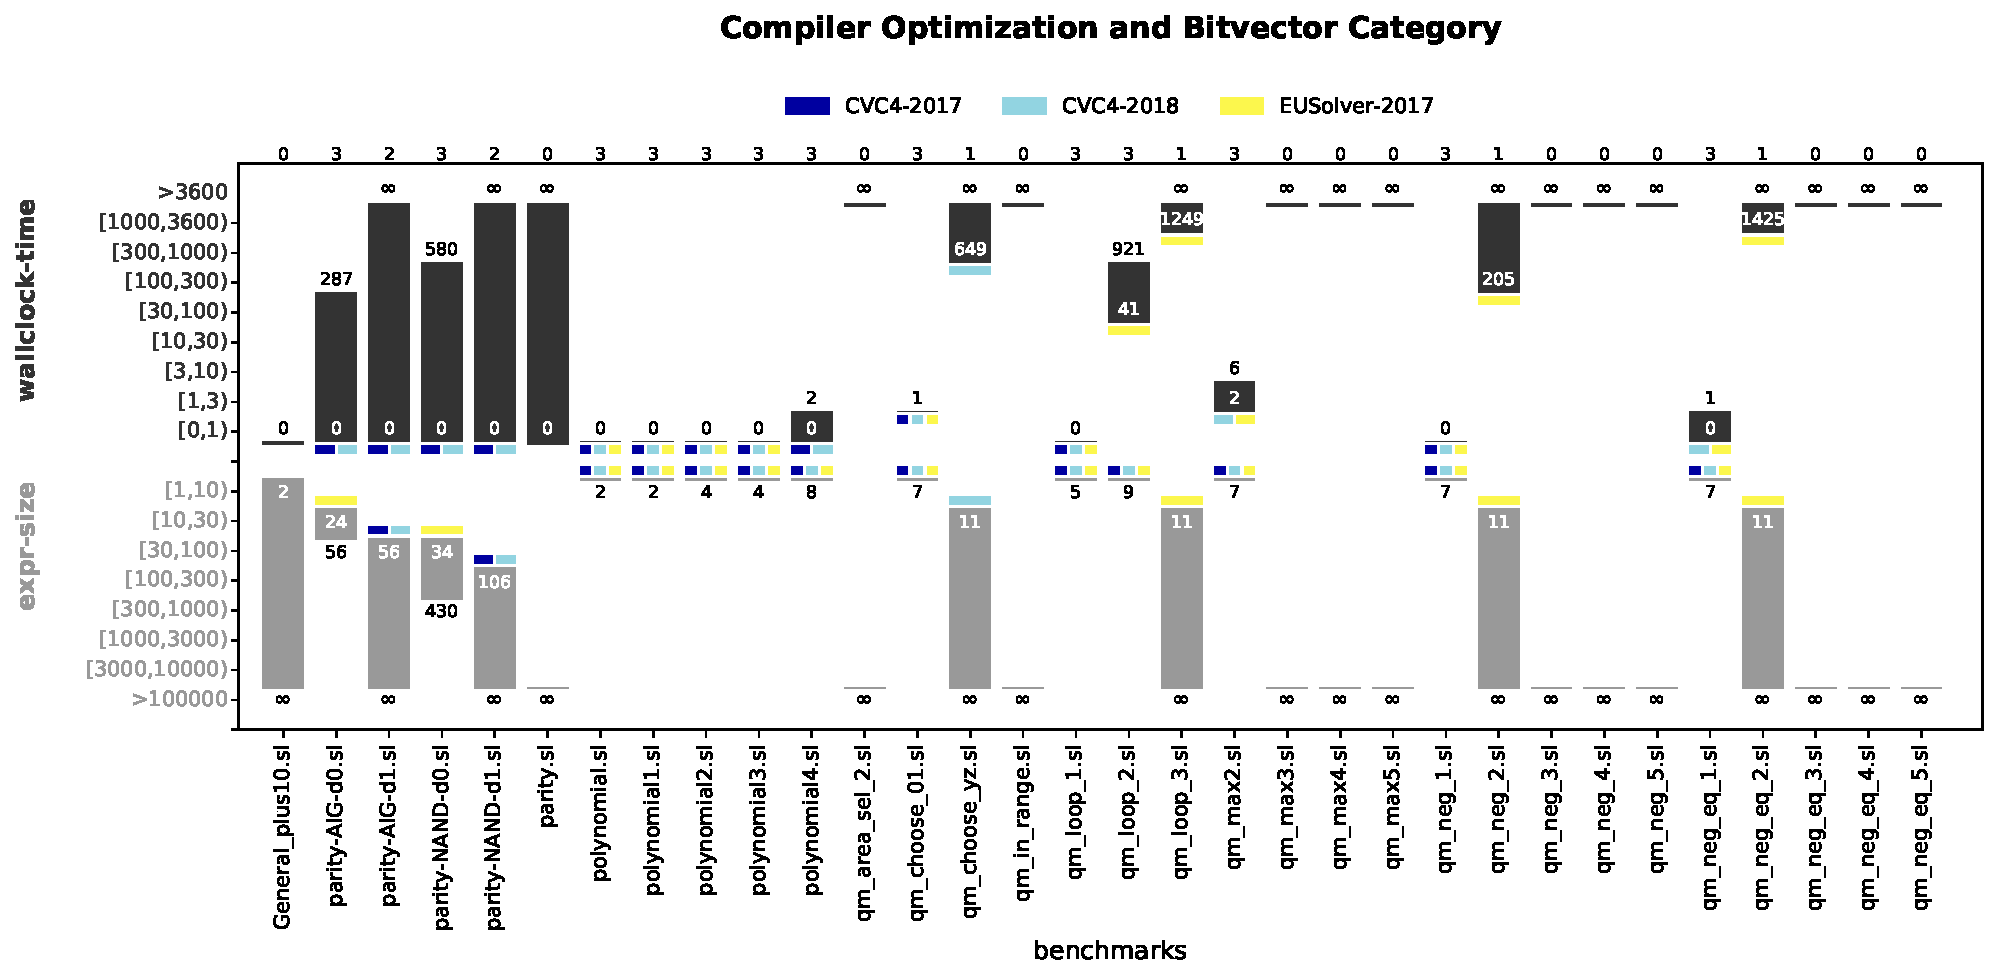
\includegraphics[width=9.5in,bb=7 9 923 476]{figures/General1.pdf} \\[3cm]
			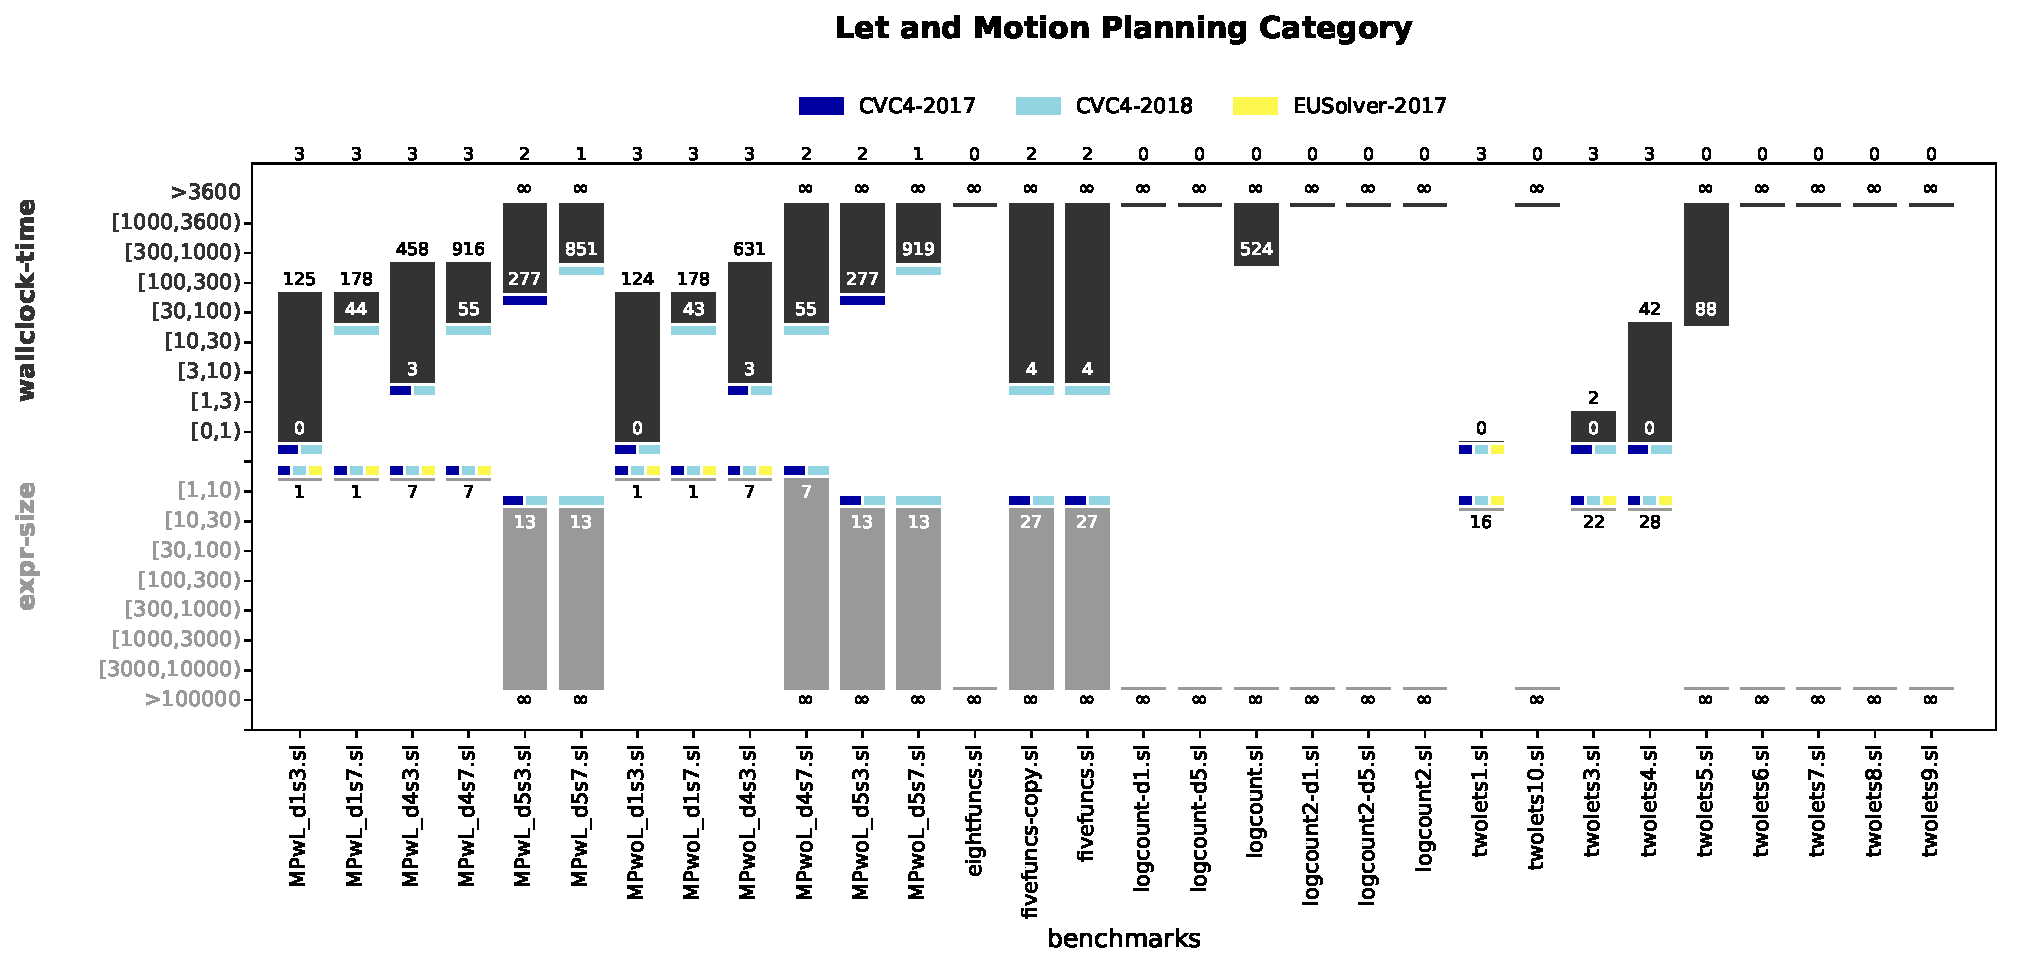
\includegraphics[width=9.5in,bb=7 9 925 460]{figures/General2.pdf} 
		\end{tabular}
	}}
	\caption{Evaluation of Compiler Optimizations, Bitvectors, Let and Motion Planning Categories of the General Track.}\label{fig:let-mot-plan}
\end{figure*}



\begin{figure*}
\noindent\makebox[\textwidth]{
	\scalebox{0.6}{
		\begin{tabular}{c}
			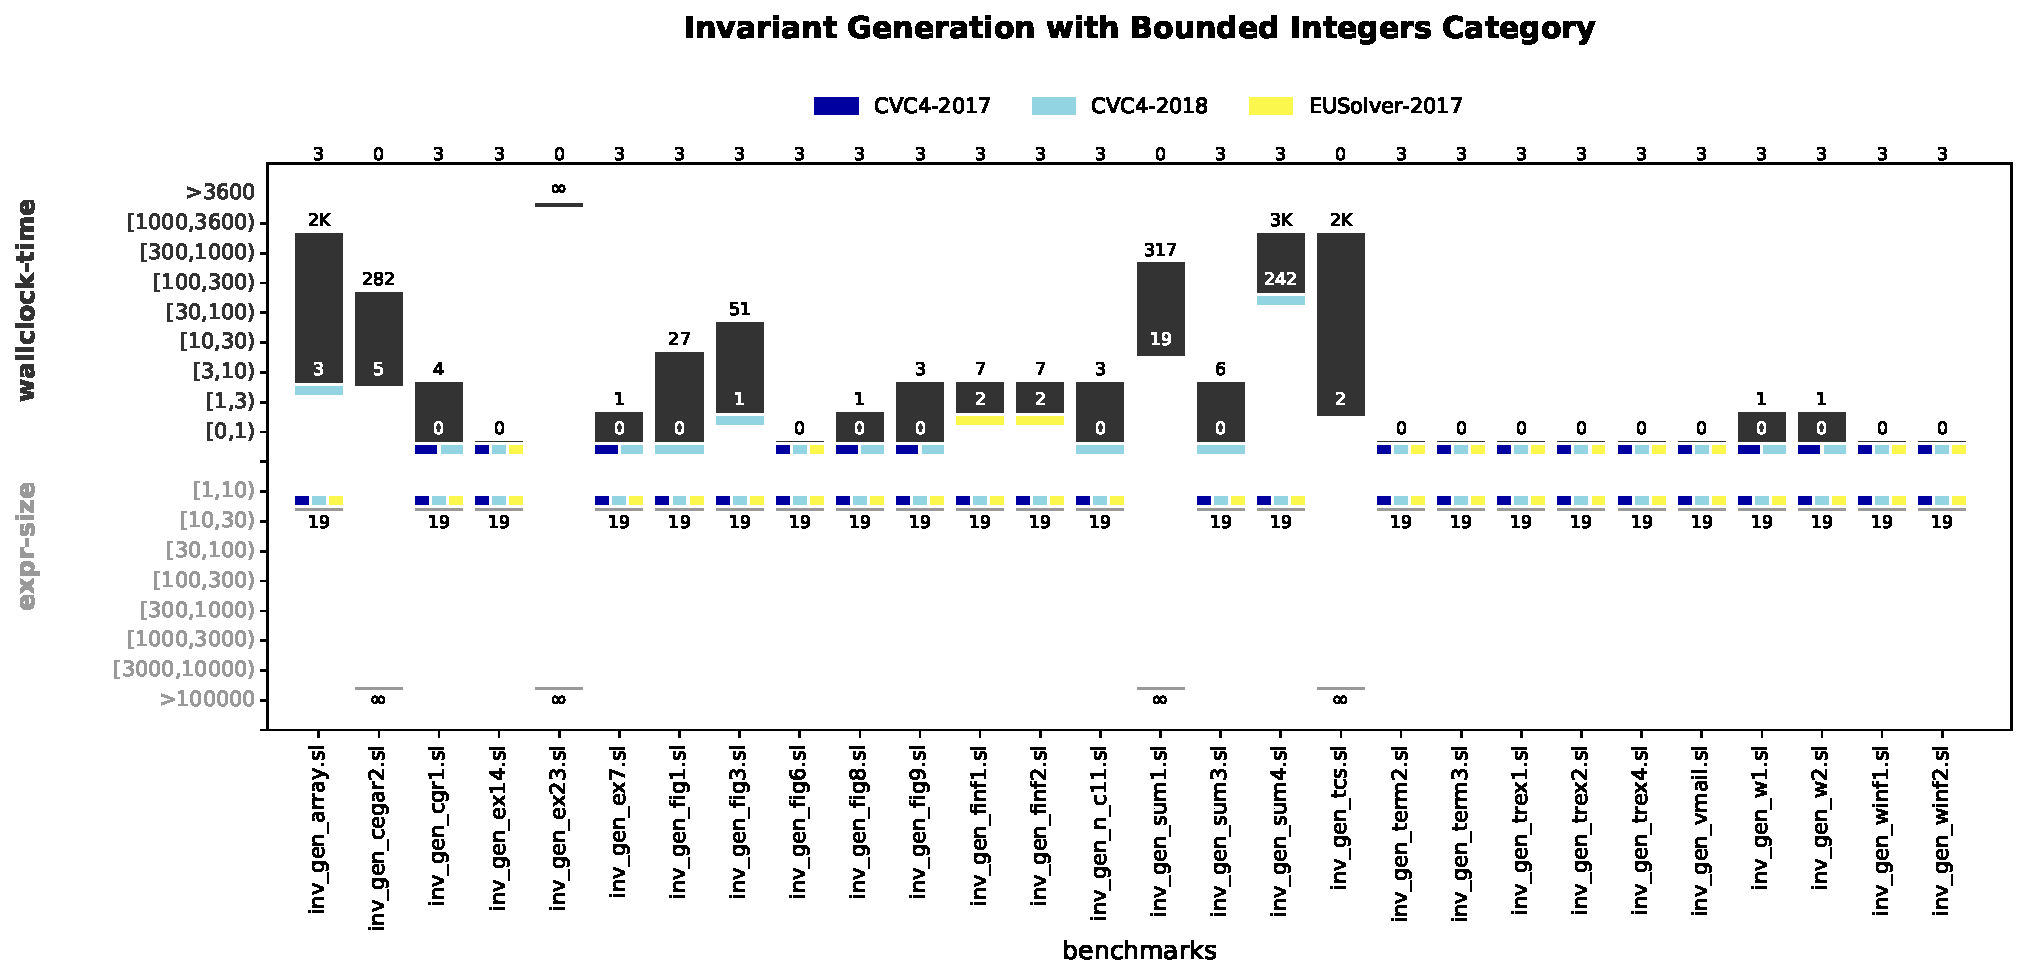
\includegraphics[width=9.5in,bb=7 9 923 476]{figures/General3.pdf} \\[3cm]
			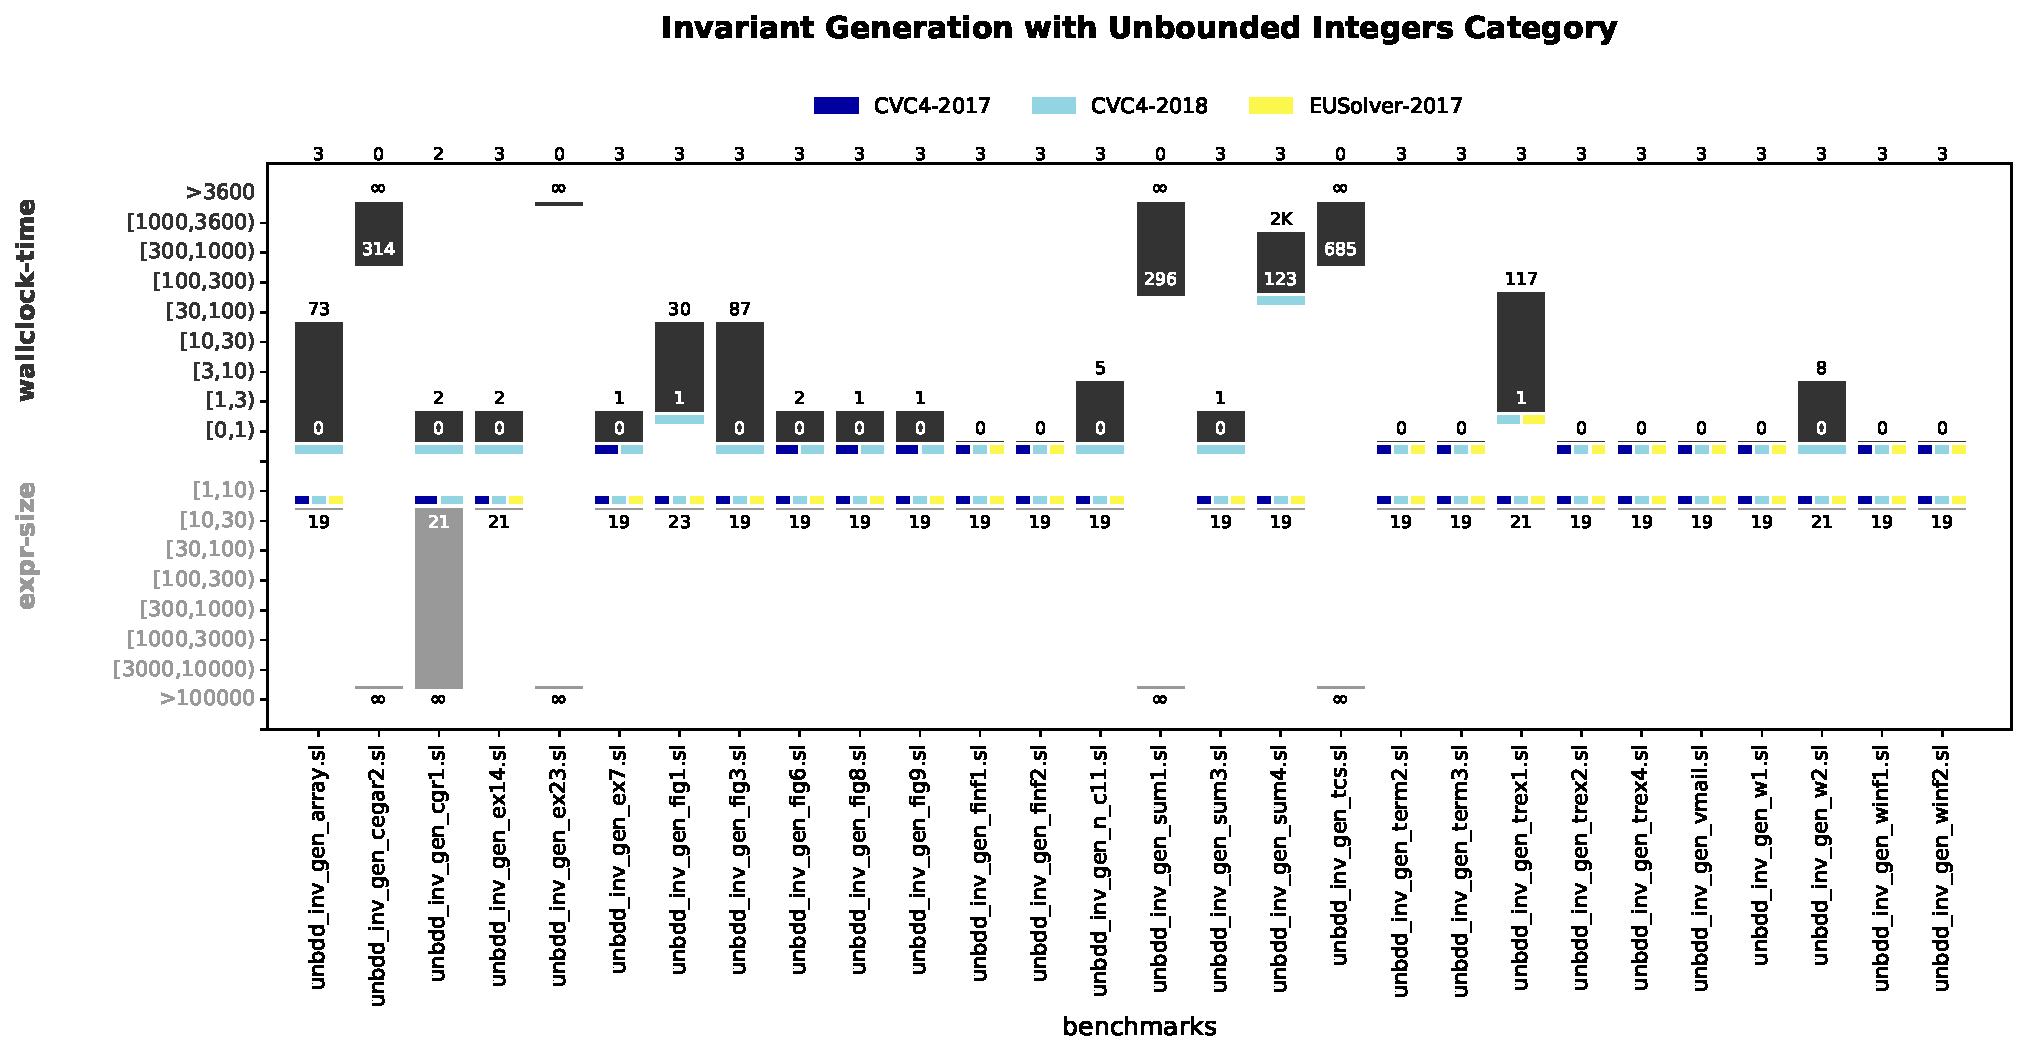
\includegraphics[width=9.5in,bb=7 9 925 460]{figures/General4.pdf} 
		\end{tabular}
	}}
	\caption{Evaluation of Invariant Generation Categories of the General Track.}\label{fig:inv-results}
\end{figure*}
		
		

		
		
\begin{figure*}
\noindent\makebox[\textwidth]{
\scalebox{0.6}{
	\begin{tabular}{c}
		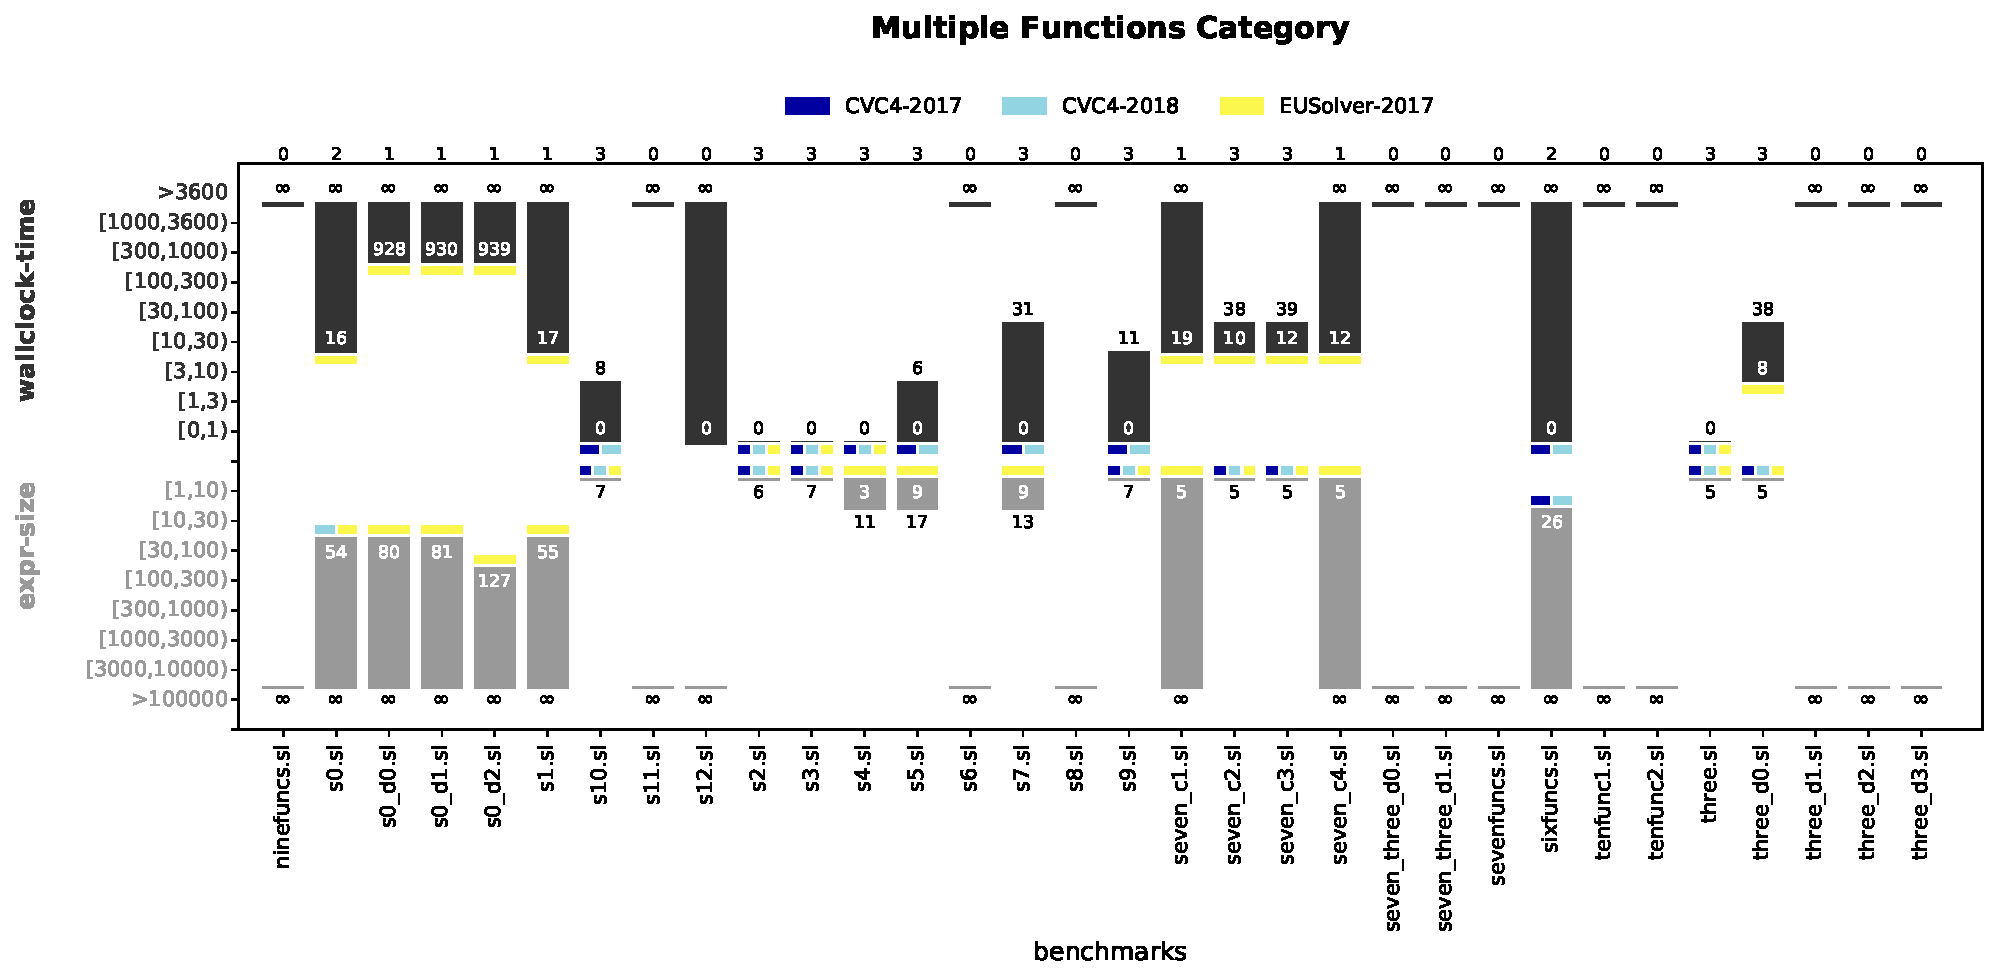
\includegraphics[width=9.5in,bb=7 9 923 476]{figures/General5.pdf} \\[3cm]
		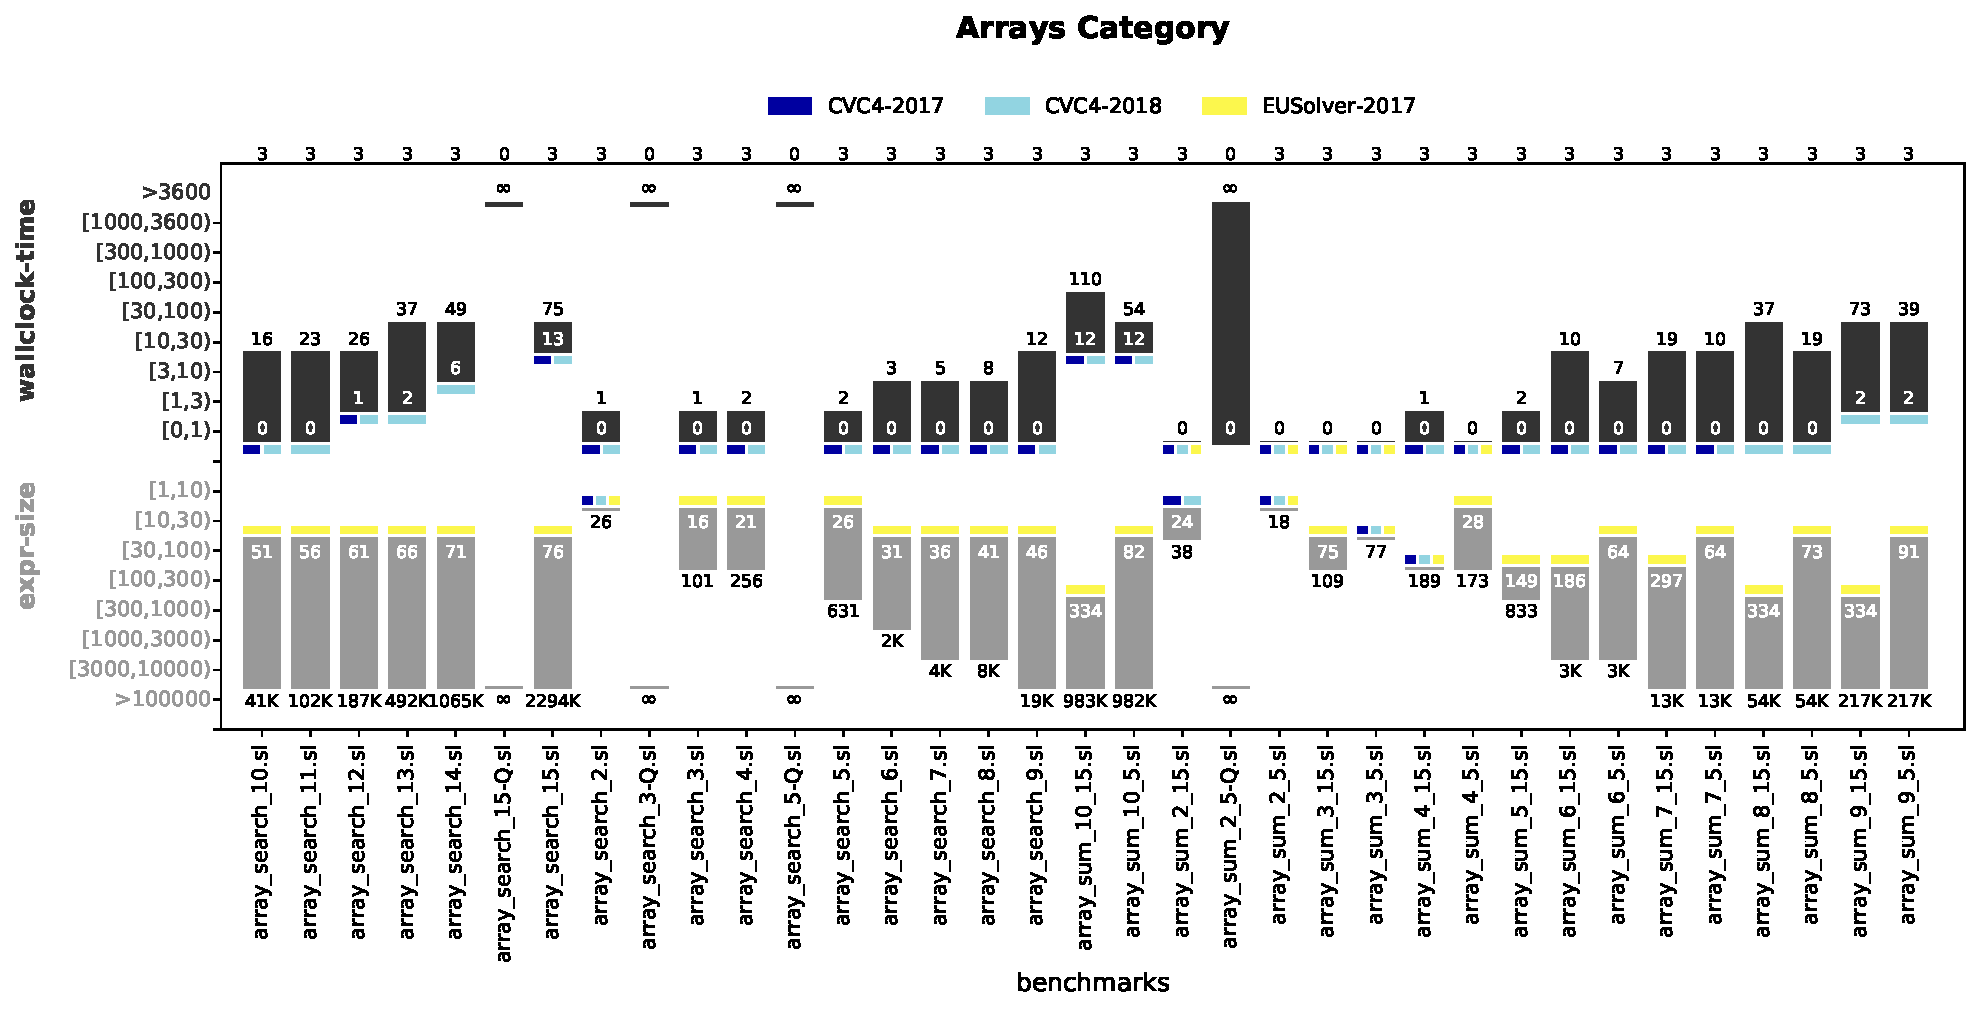
\includegraphics[width=9.5in,bb=7 9 925 460]{figures/General6.pdf} 
	\end{tabular}
}}
\caption{Evaluation of Multiple Functions and Arrays Categories of the General Track.}\label{fig:mult-func-arr}
\end{figure*}

\begin{figure*}
\noindent\makebox[\textwidth]{
	\scalebox{0.6}{
		\begin{tabular}{c}
			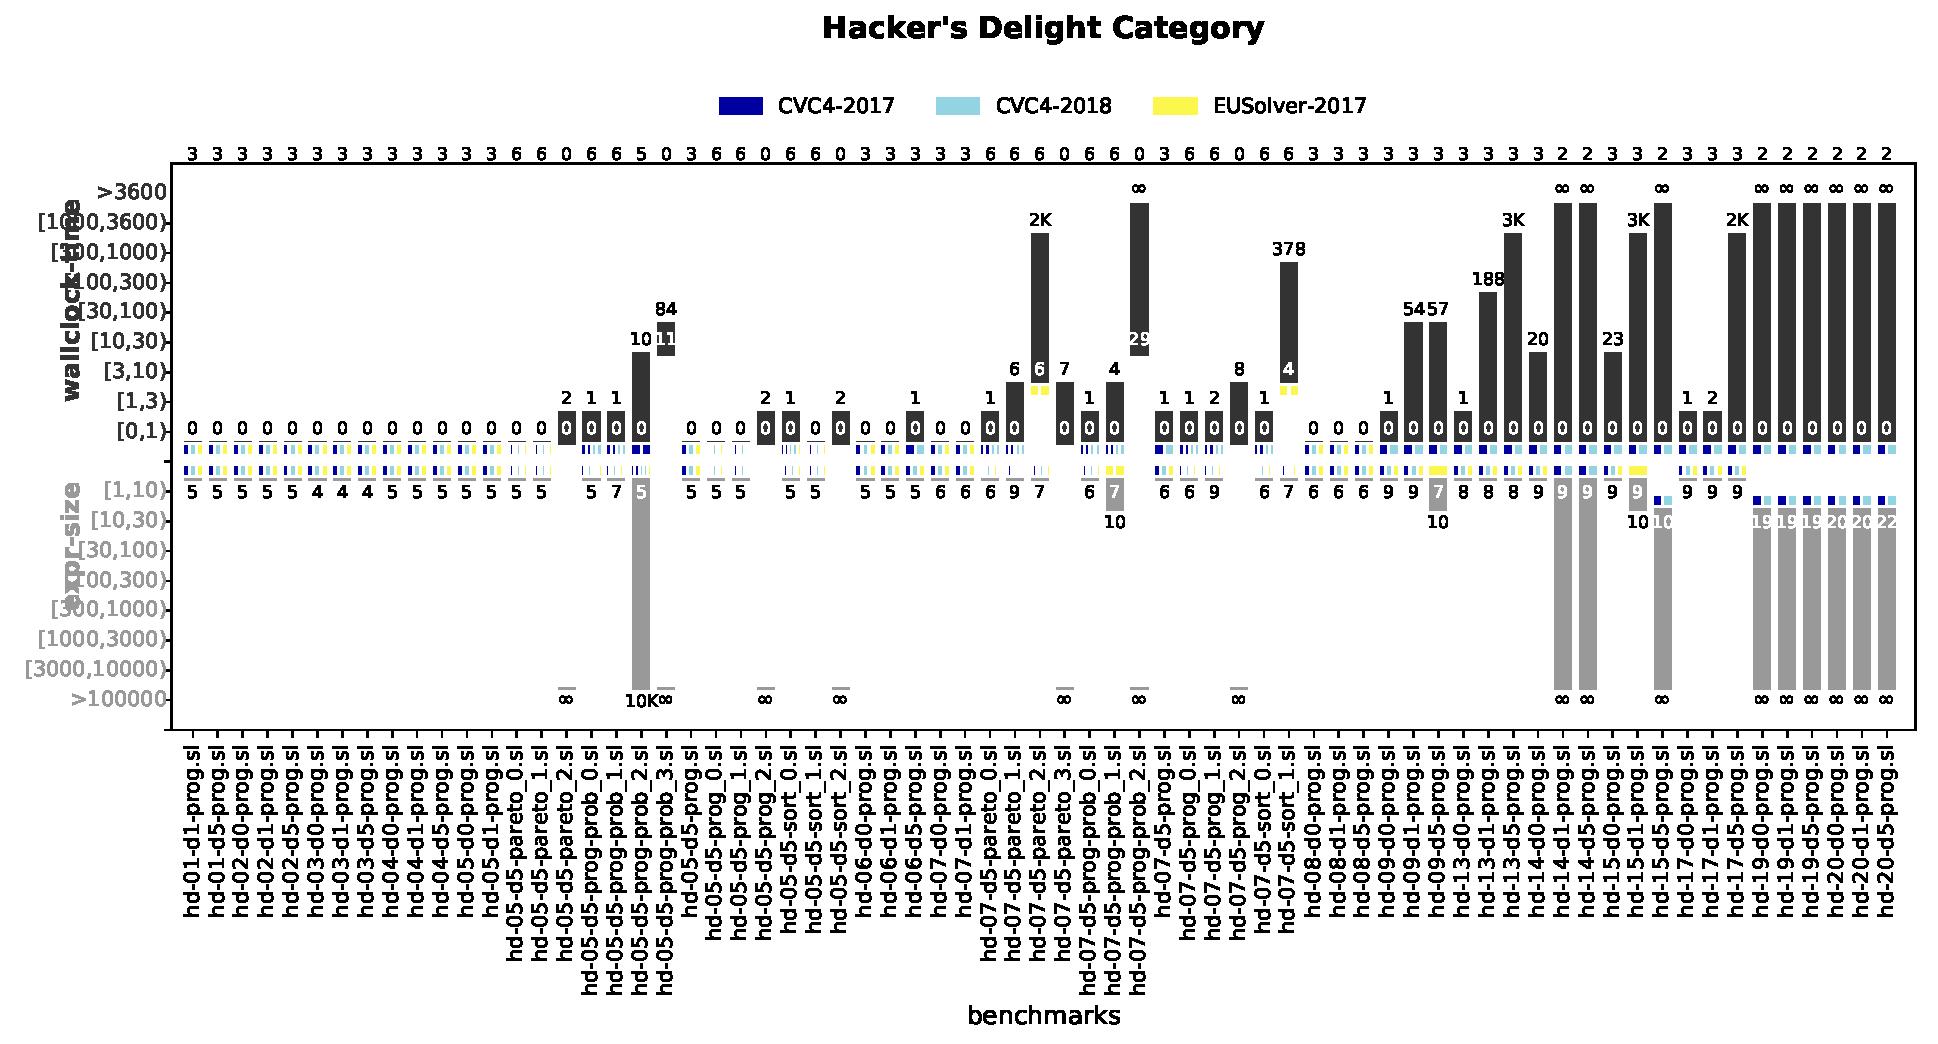
\includegraphics[width=9.5in,bb=7 9 923 476]{figures/General7.pdf} \\[3cm]
			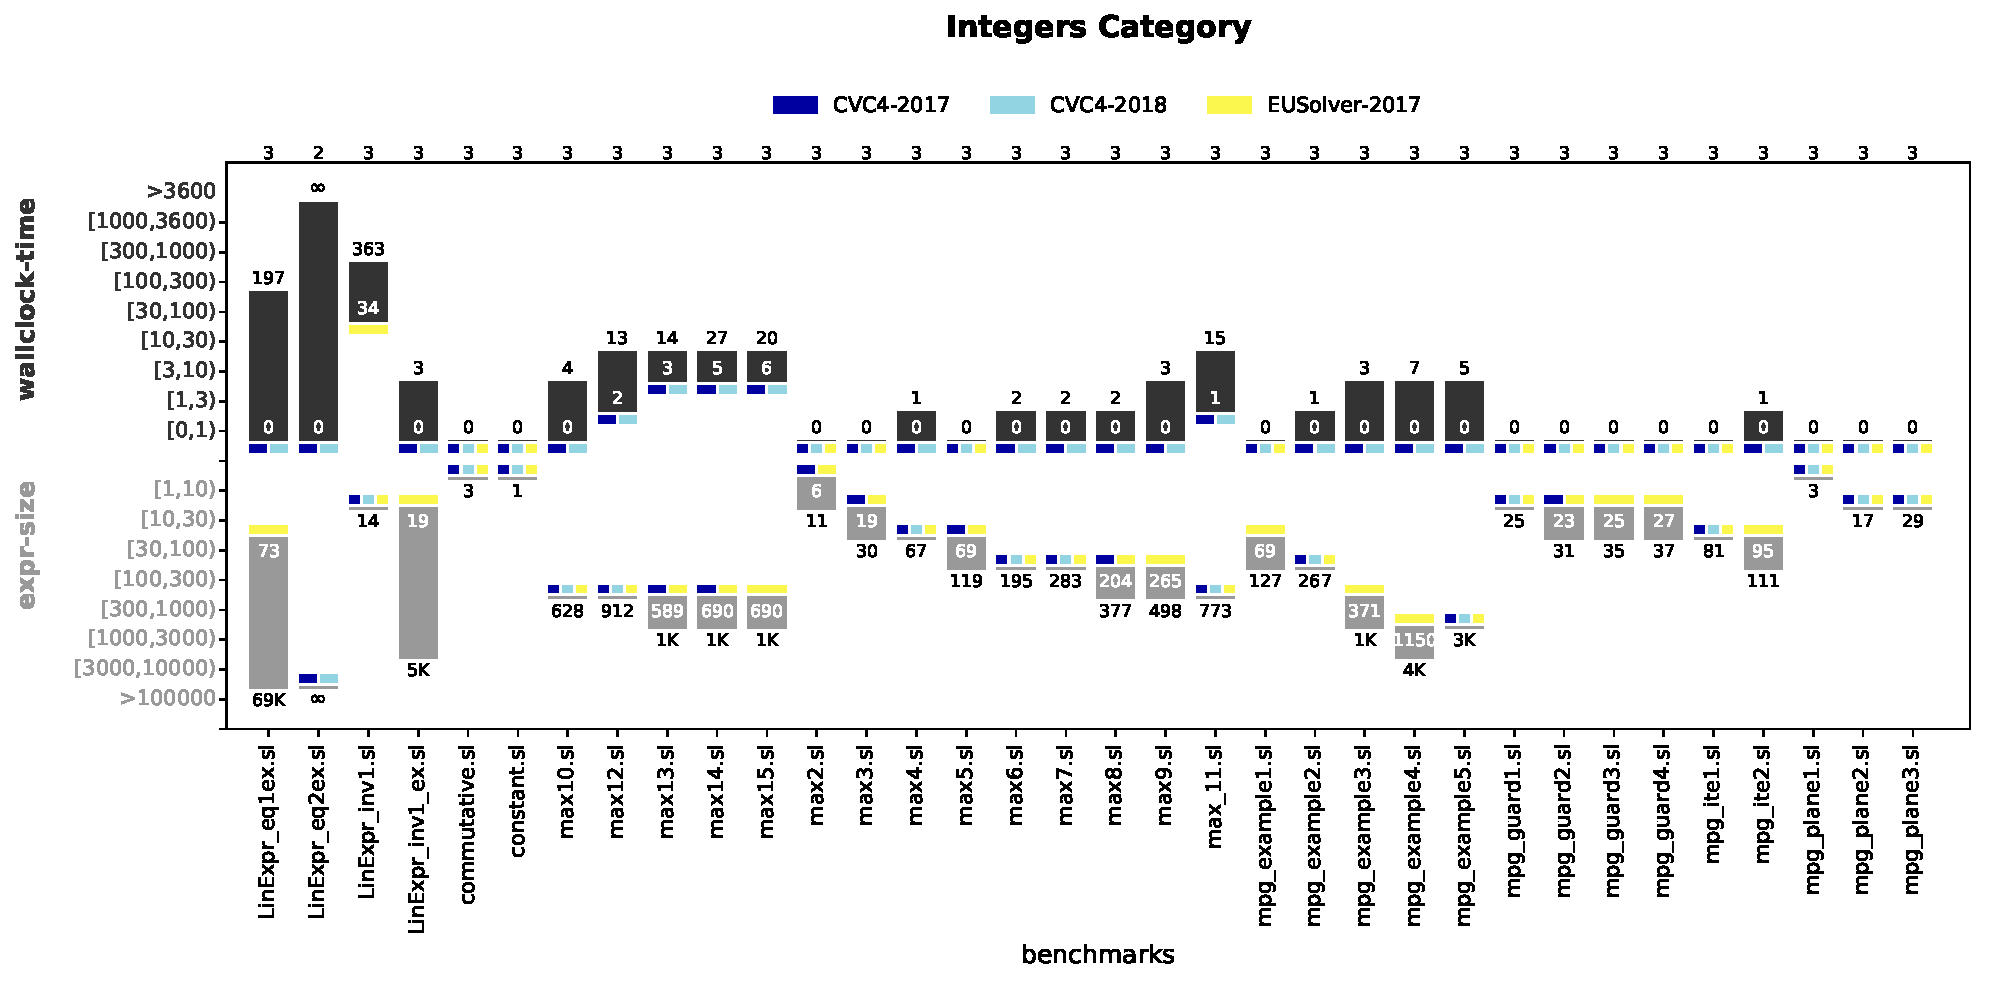
\includegraphics[width=9.5in,bb=7 9 925 460]{figures/General8.pdf} 
		\end{tabular}
	}}
	\caption{Evaluation of Hacker's Delight and Integers Categories of the General Track.}\label{fig:hd-int}
\end{figure*}
				

				
\begin{figure*}
\noindent\makebox[\textwidth]{
\scalebox{0.6}{
	\begin{tabular}{c}
		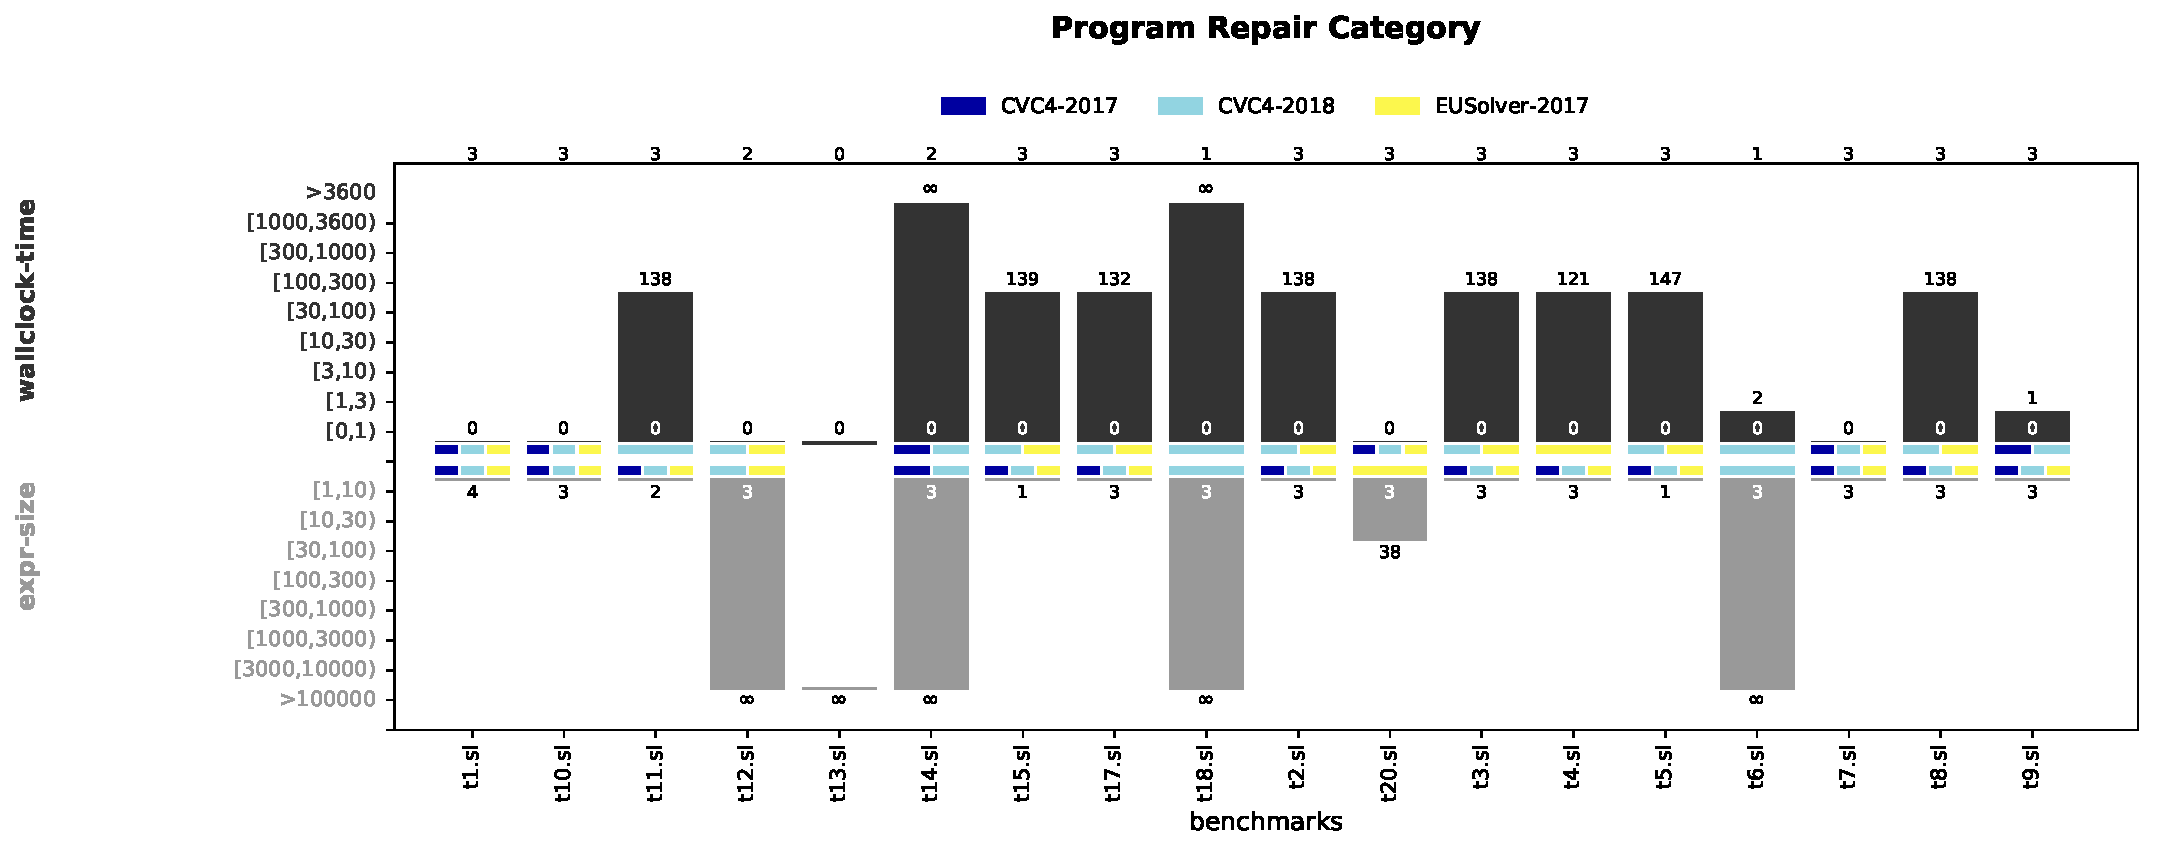
\includegraphics[width=9.0in,bb=7 9 923 476]{figures/General9.pdf} \\[3cm]
		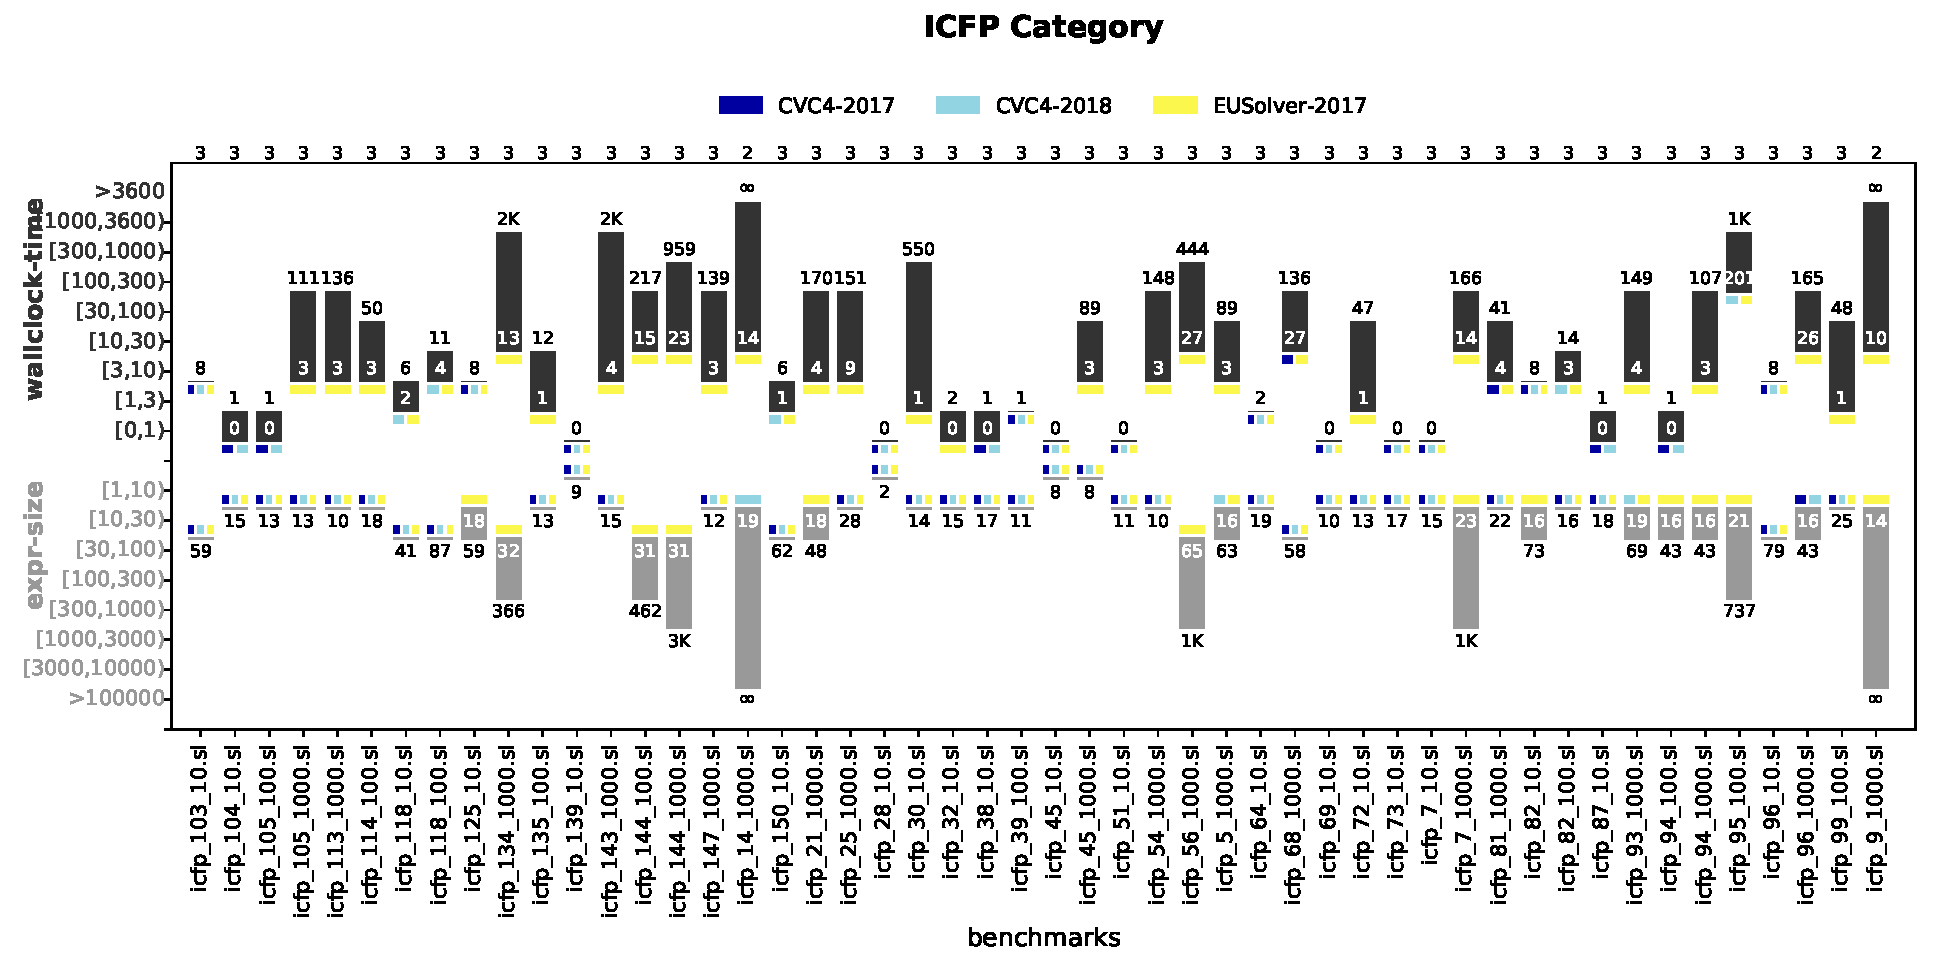
\includegraphics[width=9.7in,bb=7 9 925 460]{figures/General10.pdf} 
	\end{tabular}
}}
\caption{Evaluation of Program Repair and ICFP Categories of the General Track.}\label{fig:prog-rep-icfp}
\end{figure*}



\begin{figure*}
\noindent\makebox[\textwidth]{
	\scalebox{0.6}{
		\begin{tabular}{c}
			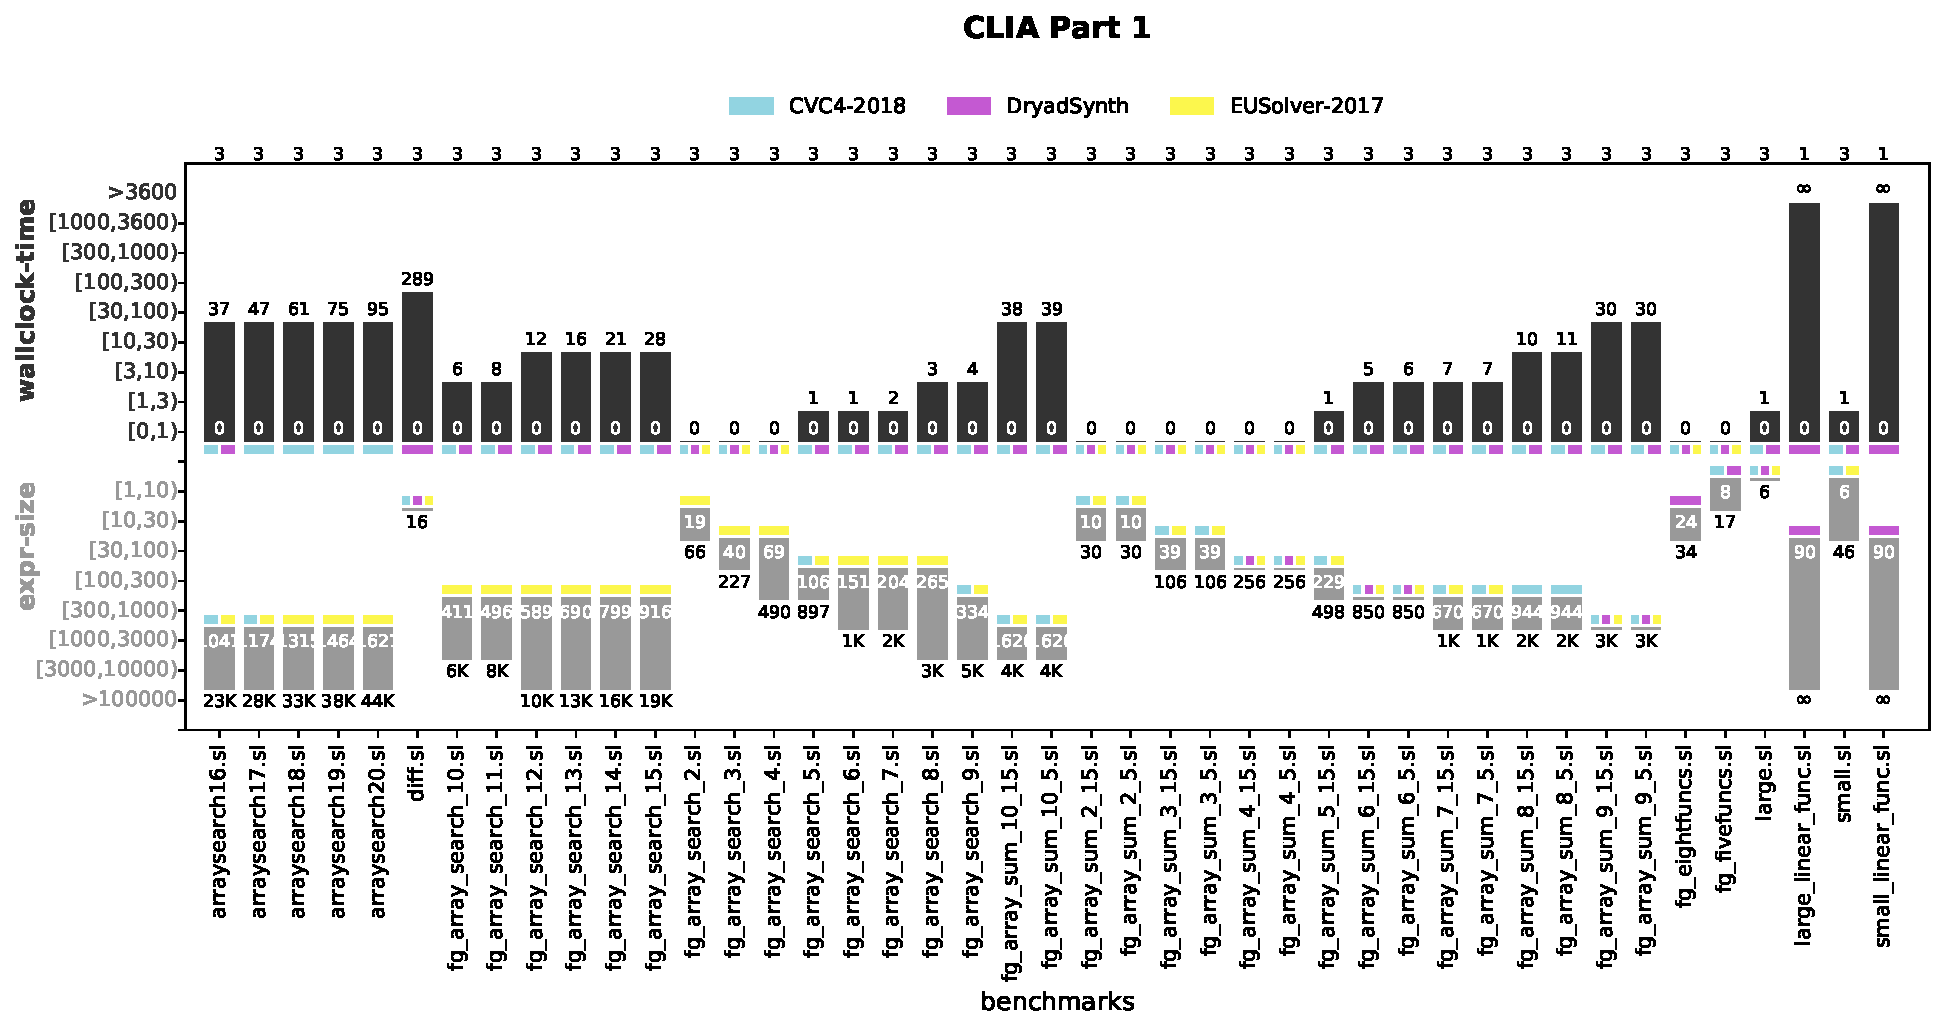
\includegraphics[width=9.5in,bb=7 9 923 476]{figures/CLIA1.pdf} \\[3cm]
			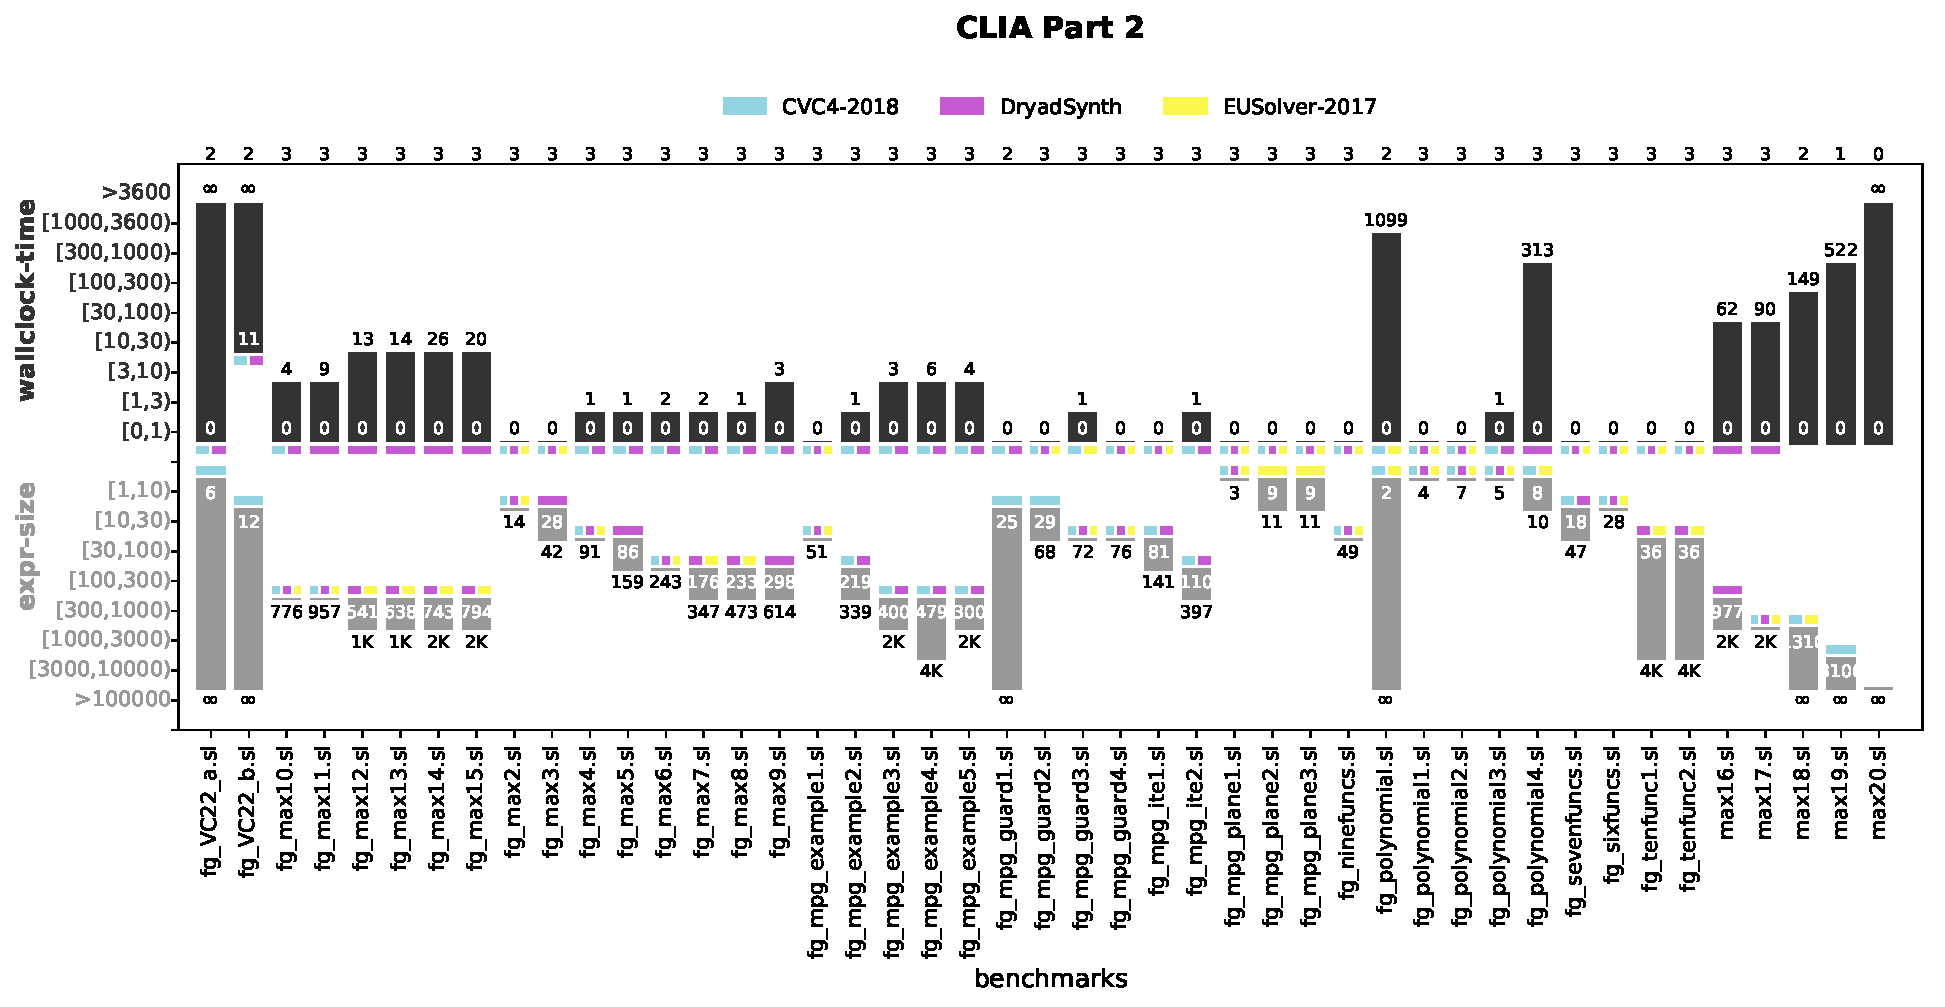
\includegraphics[width=9.5in,bb=7 9 925 460]{figures/CLIA2.pdf} 
		\end{tabular}
	}}
	\caption{Evaluation of CLIA track benchmarks.}\label{fig:clia-results}
\end{figure*}
	


\begin{figure*}
\noindent\makebox[\textwidth]{
	\scalebox{0.6}{
		\begin{tabular}{c}
			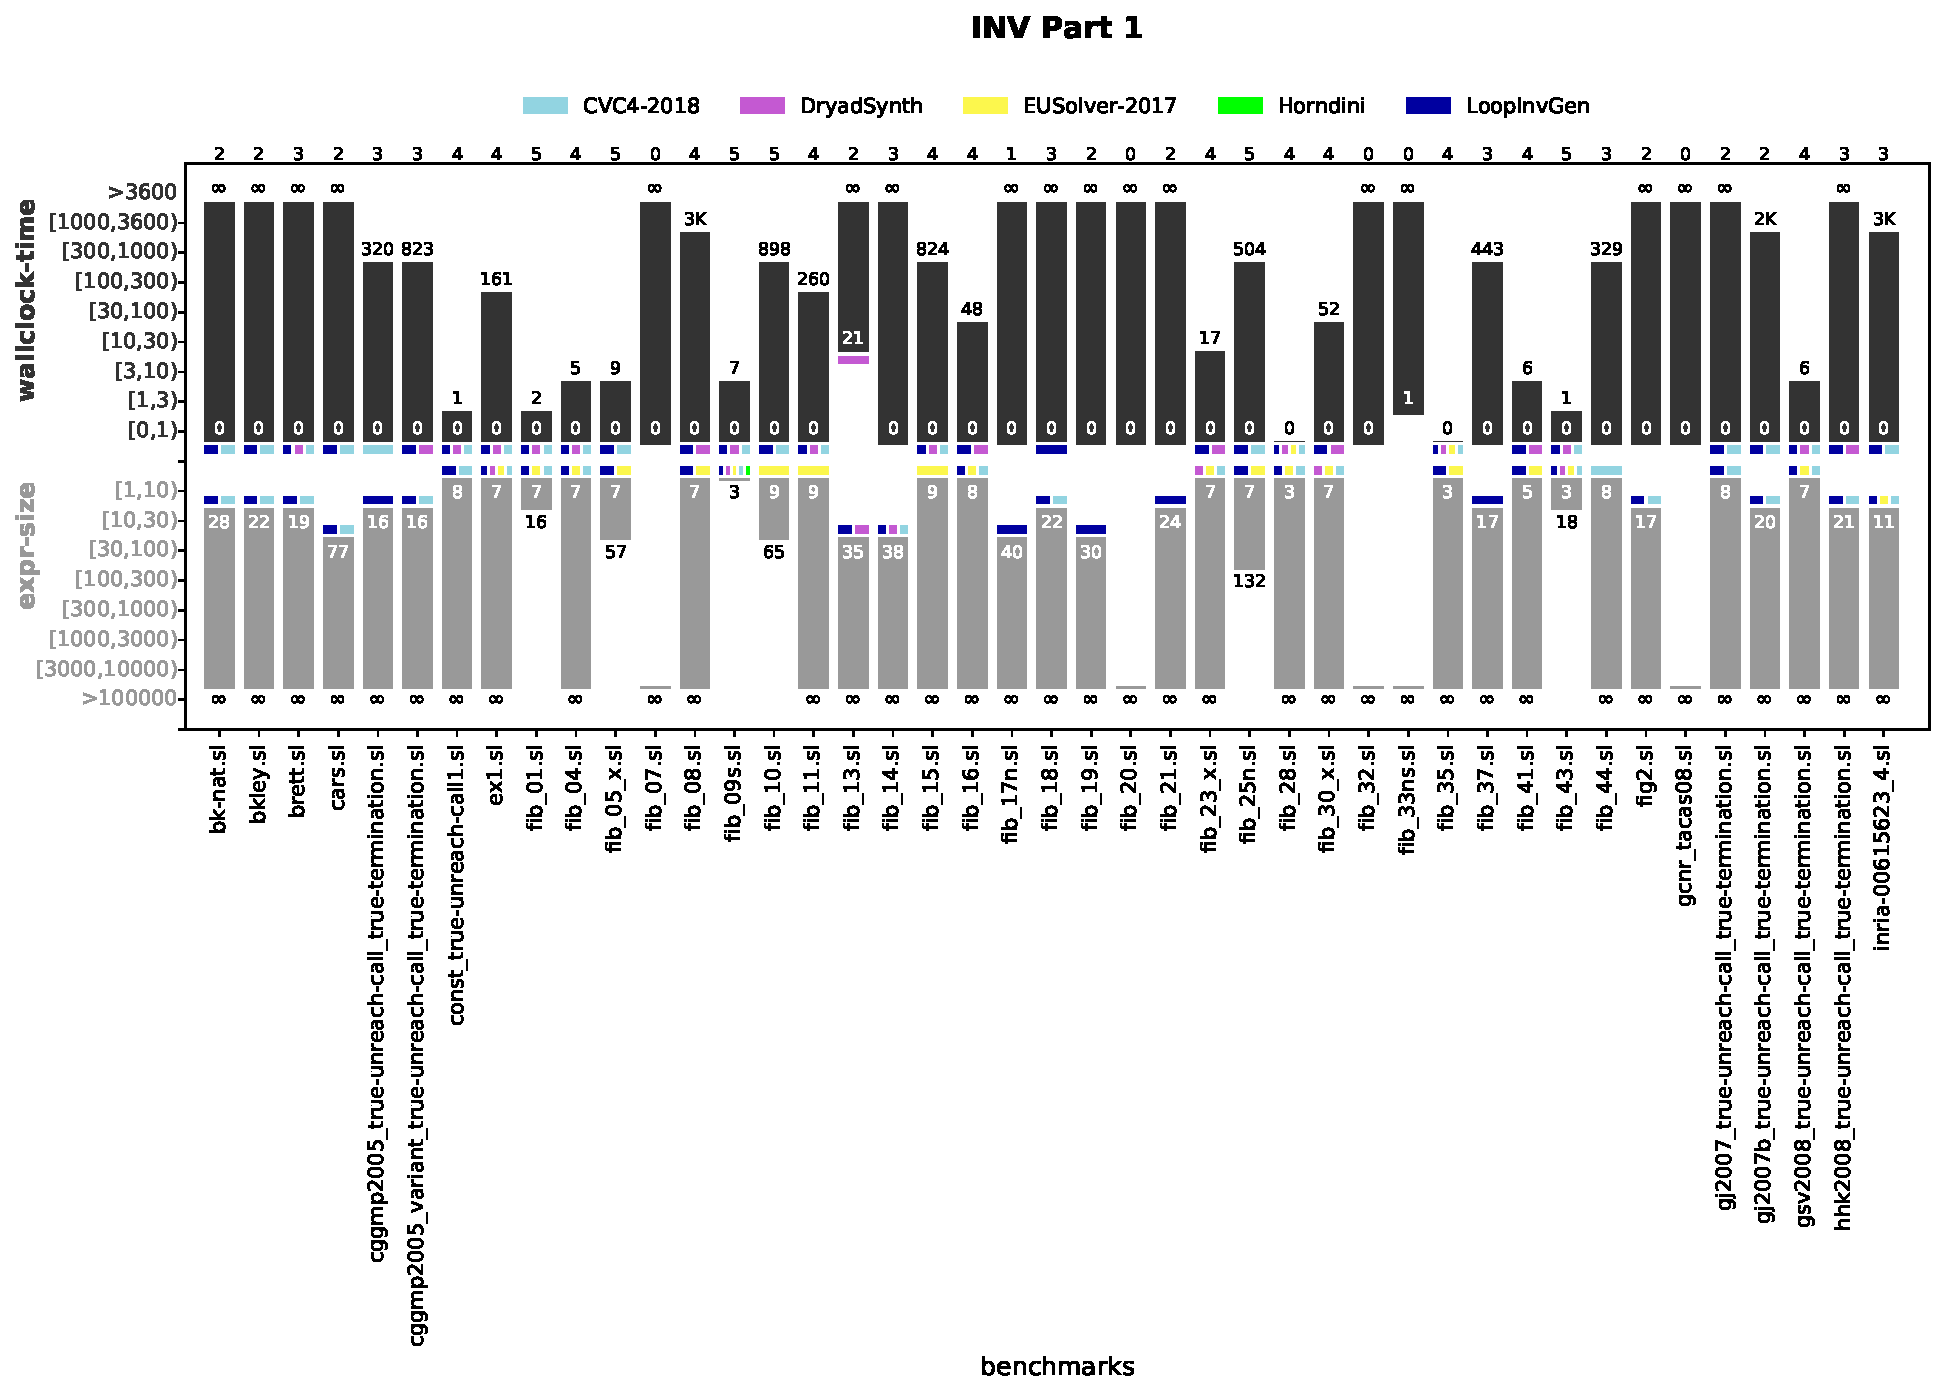
\includegraphics[width=9.5in]{figures/Inv1.pdf} \\[1cm]
			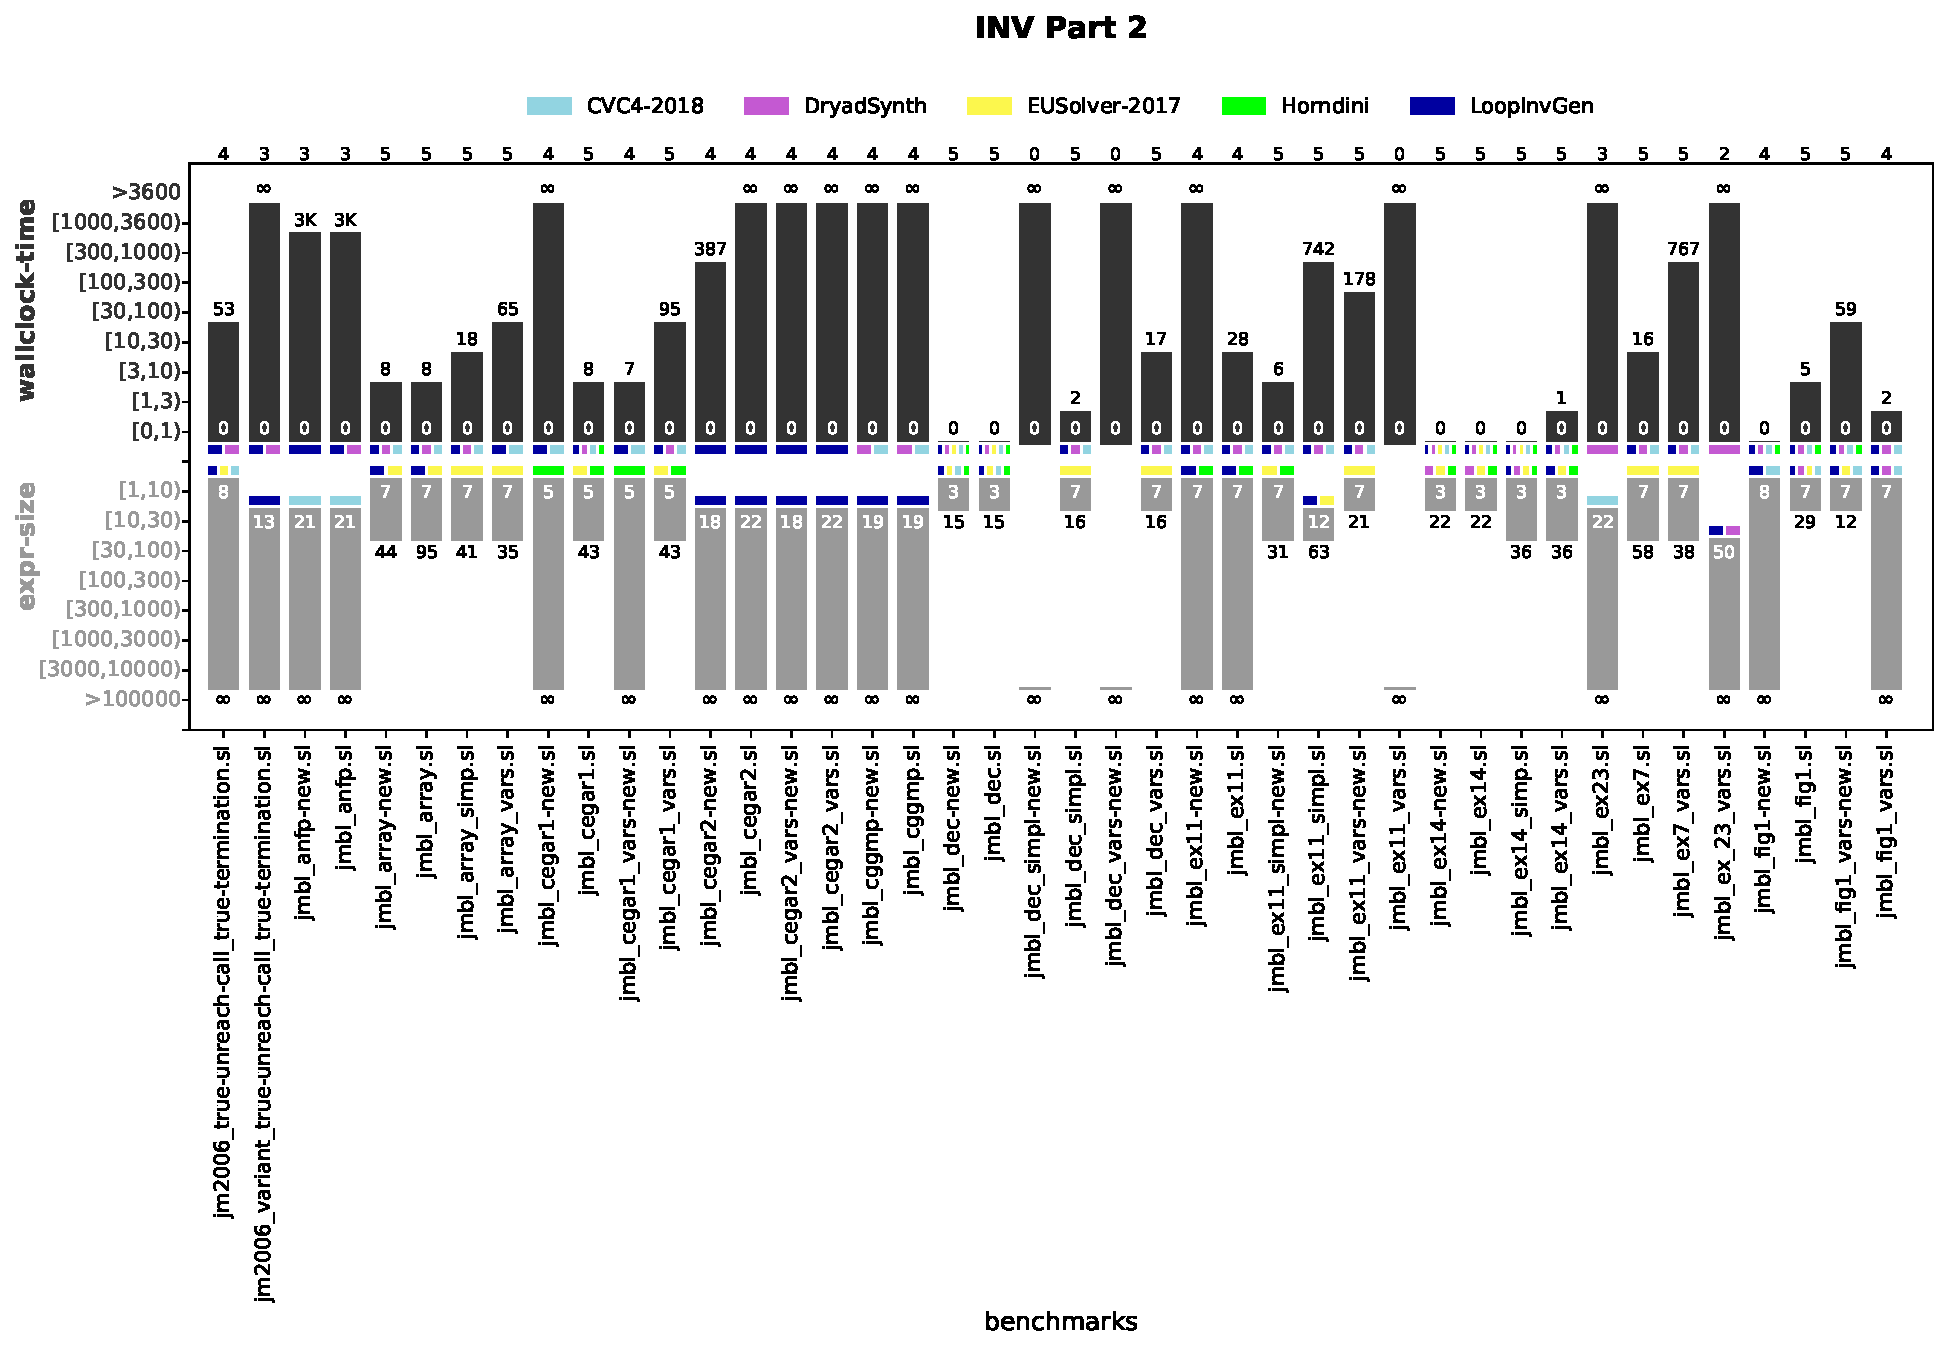
\includegraphics[width=9.5in]{figures/Inv2.pdf} \\[1cm]
			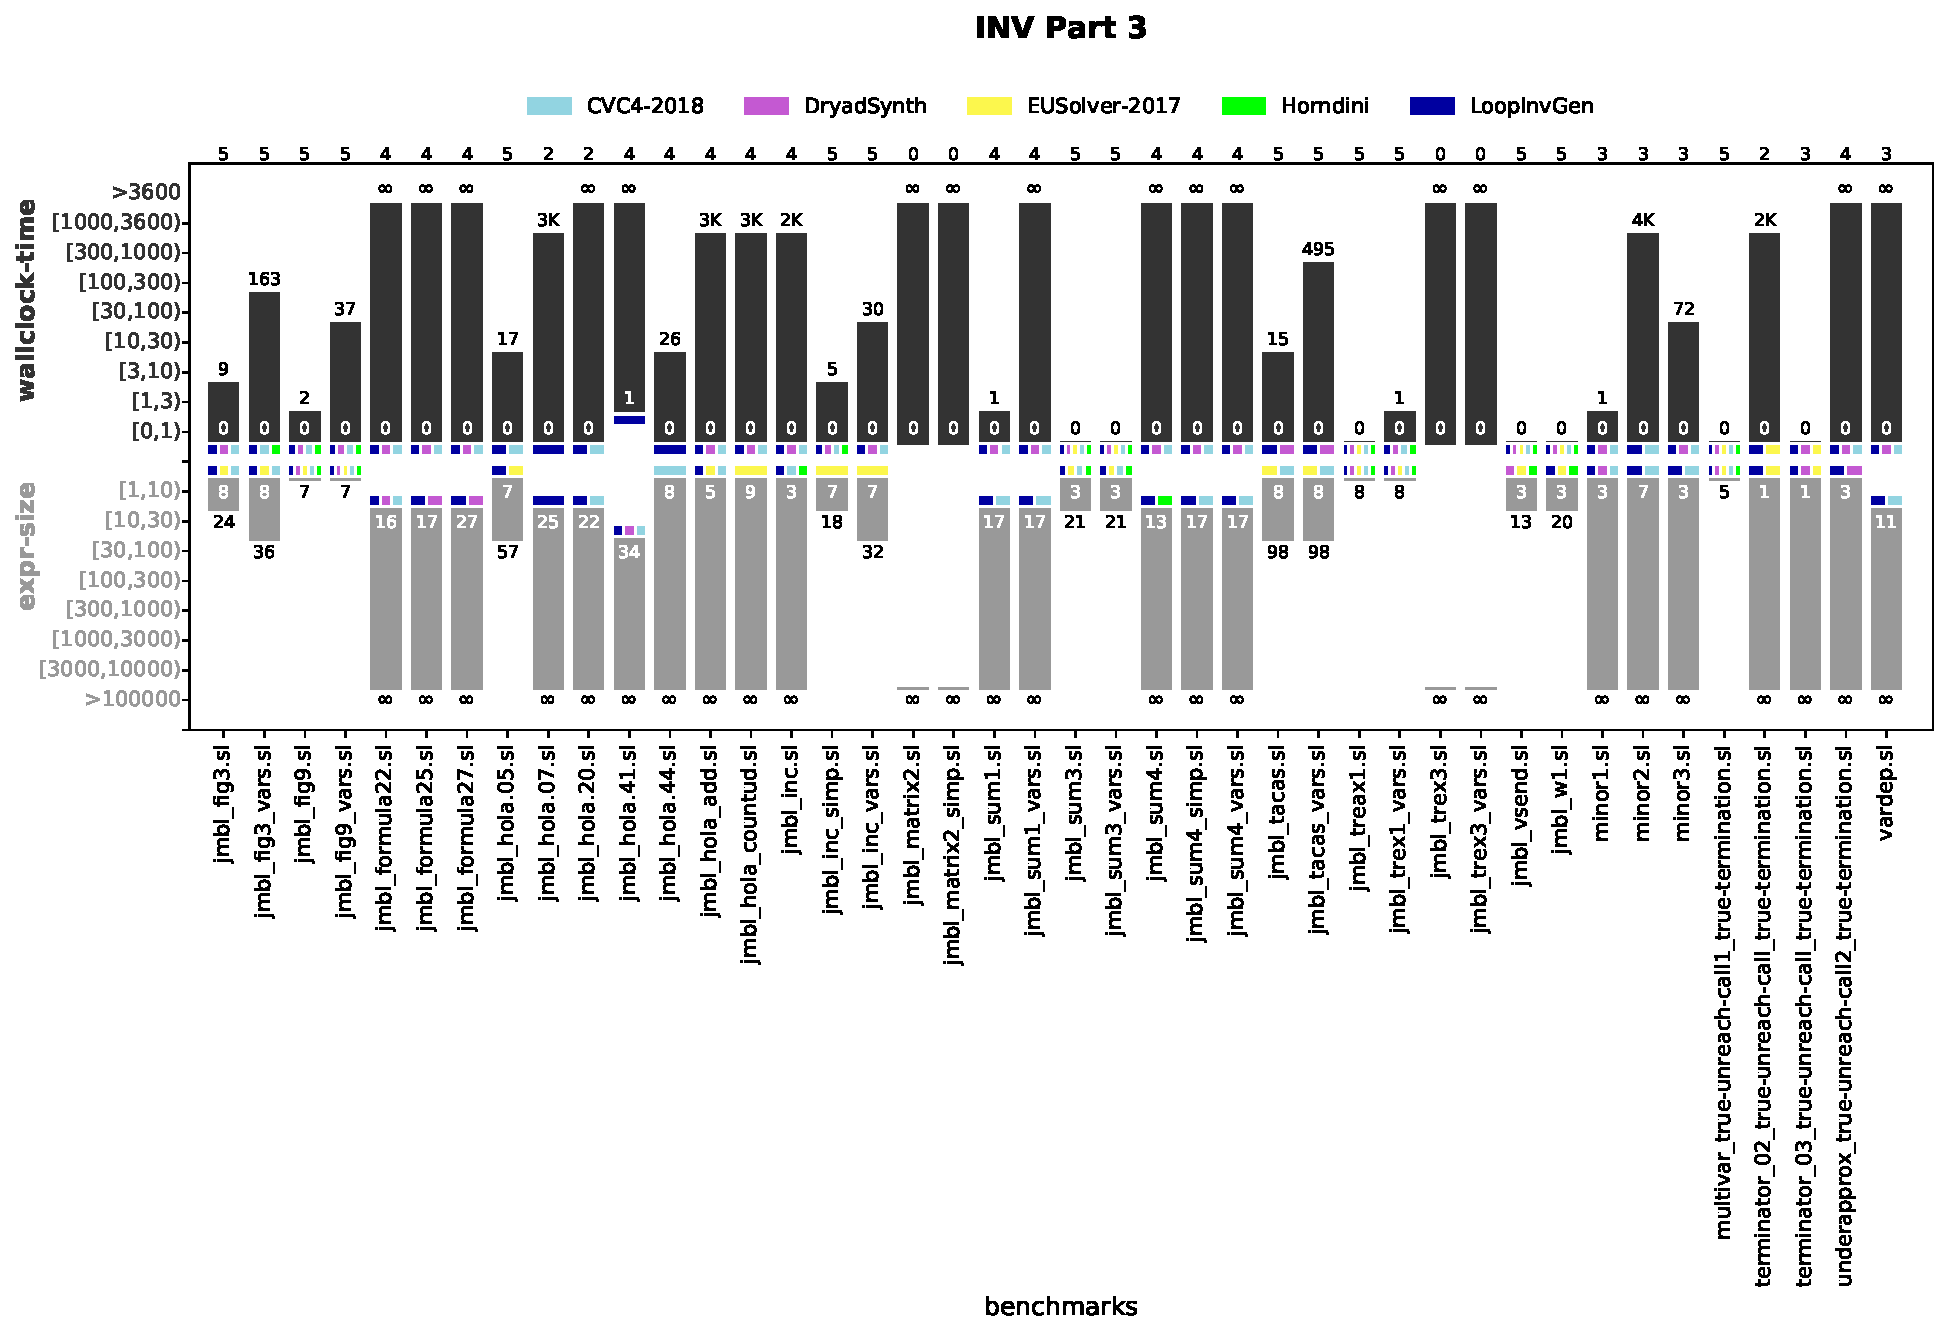
\includegraphics[width=9.5in]{figures/Inv3.pdf}
		\end{tabular}
	}}
	\caption{Evaluation of Invariant track benchmarks.}\label{fig:inv-results}
\end{figure*}



\begin{figure*}
\noindent\makebox[\textwidth]{
	\scalebox{0.6}{
		\begin{tabular}{c}
			\includegraphics[width=9.5in,bb=7 9 923 476]{Figures/FigPBEStringsRevPart1.pdf} \\[3cm]
			\includegraphics[width=9.5in,bb=7 9 925 460]{Figures/FigPBEStringsRevPart2.pdf} 
		\end{tabular}
	}}
	\caption{Evaluation of PBE Strings track benchmarks.}\label{fig:pbe-strings-results}
\end{figure*}



